\documentclass{article}
% Package to manage page layout
\usepackage[margin=1.5cm, includefoot, footskip=30pt]{geometry}

\setlength\parindent{0pt}
\setlength{\parskip}{1em}

%%%%%%%PACKAGES HERE%%%%%%%
\usepackage{amsmath}
\usepackage{amsthm}
\usepackage{amssymb}
\usepackage{hyperref}
\usepackage{standalone}
\usepackage{subcaption}
\usepackage{adjustbox}
\usepackage{tikz}
\usepackage{booktabs}
\usepackage{minted}
\usepackage{multicol}
\usepackage{graphicx}
\usepackage{algorithm,algorithmic}
\usetikzlibrary{er,positioning, calc}

\definecolor{background}{RGB}{5, 66, 81}
\usemintedstyle{tango}

\setcounter{secnumdepth}{4}
\setcounter{tocdepth}{4}

\usepackage{kbordermatrix}
\theoremstyle{definition}
\newtheorem{definition}{Definition}[section]

%%%%%%%%%%%%%%%%%%%%%%%%%%%%%%%PARAMETERS%%%%%%%%%%%%%%%%%%%%%%%%%%%%%%%%%%%%%%%
\newcommand{\totalarticles}{\input{assets/total_articles.txt}}
\newcommand{\manual}{\input{assets/prov_manual.txt}}
\newcommand{\authors}{\input{assets/number_of_authors.txt}}
\newcommand{\edges}{\input{assets/pd_edges.txt}}
\newcommand{\isolated}{\input{assets/isolated_authors.txt}}
\newcommand{\isolatedpercentage}{\input{assets/isolated_authors_percentage.txt}}
\newcommand{\connectedcomponents}{\input{assets/number_of_connected.txt}}
\newcommand{\largestcc}{\input{assets/largest_cc.txt}}
\newcommand{\clustering}{\input{assets/clustering_coeff.txt}}
\newcommand{\avdegree}{\input{assets/av_degree.txt}}
% \newcommand{\prisonerscc}{\input{assets/prisoners_clustering.txt}}
% \newcommand{\pricecon}{162}
% \newcommand{\pricecc}{0.71}
% \newcommand{\auctioncon}{\input{assets/auction_connected_components.txt}}
% \newcommand{\auctioncc}{\input{assets/auction_clustering.txt}}
% \newcommand{\prisonerisolated}{\input{assets/prisoners_isolated.txt}}
% \newcommand{\auctionisolated}{\input{assets/auction_isolated.txt}}
% \newcommand{\priceisolated}{\input{assets/price_isolated.txt}}
%%%%%%%%%%%%%%%%%%%%%%%%%%%%%%%%%%%%%%%%%%%%%%%%%%%%%%%%%%%%%%%%%%%%%%%%%%%%%%%%
%%%%%%%%%%%%%%%%%%%%%%%%%%%%%%%%%%%%%%%%%%%%%%%%%%%%%%%%%%%%%%%%%%%%%%%%%%%%%%%%
\title{A systematic literature review of the Prisoner's Dilemma; collaboration and influence.}
\author{Nikoleta E. Glynatsi, Vincent A. Knight}
\date{}

\begin{document}

\maketitle

% \begin{abstract}
%     The emergence of cooperation is a topic of continuing interest
%     for social, biological and ecological sciences. The game called the prisoner's
%     dilemma has been used ever since the 1950's as a framework for studying the emergence
%     of cooperation. The iterated version of the game attracted attention in 1980's after
%     the publication of the ``The Evolution of Cooperation'' and has been a topic
%     of pioneering research ever since. In this work we aim to provide a chronological
%     literature review of the field. This is achieved by partitioning the timeline into five different
%     time periods. Furthermore, a comprehensive data set of literature was analysed
%     using network theoretic approaches in order to explore the collaborative
%     behaviour and identify the influencers of the field.
% \end{abstract}

% \section{The Prisoner's Dilemma}\label{section:introduction}

% The prisoner's dilemma is a two player non-cooperative game, originally described in~\cite{Flood1958} where
% the decisions of the players are made simultaneously and independently. Both players
% can choose between cooperation (\textbf{C}) or defection (\textbf{D}).

% The fitness of each player is influenced by its own behaviour, and the behaviour
% of the opponent. If both players choose to cooperate, both do better
% than if both defect. However, a player has the temptation to deviate. If a
% player was to defect while the other cooperates, the defector receives
% more than if both had cooperated. The reward for mutual cooperation is \(R\),
% for a mutual defection they receive \(P\), and for cooperation-defection,
% the cooperator receives \(S\) where the defector receives \(T\). The game's
% payoffs are generally represented by,

% \begin{equation} \label{eq:the_pd_payoffs}
%     \begin{pmatrix}
%     R & S \\ T & P
%     \end{pmatrix}
% \end{equation}

% where \(T > R > P > S \) and \(2R > T + S\) are the conditions for a dilemma
% to exist. Due to rational behaviour and the knowledge that an individual is tempted
% to defect the game's equilibrium lies at mutual defection and both players
% receive a payoff of \(P\). Thus, the dominant strategy for the prisoner's dilemma
% is \textbf{D}.

% When the game is studied in a manner where prior outcomes matter, the
% defecting choice is no longer necessarily the dominant choice. The repeated
% form of the game is called the iterated prisoner's dilemma and now two players play
% the game repeatedly. Interest was sparked on the iterated prisoner dilemma by
% R. Axelrod and his book~\cite{Axelrod1984} ``The Evolution of Cooperation''.

% In his book Axelrod reports on a series of computer tournaments he organised of
% a finite turns games of the iterated prisoner's dilemma. Participants
% had to choose between \textbf{C} and \textbf{D} again and again while having
% memory of their previous encounters. Academics from several fields were invited to
% design computer strategies to compete in the tournament. The pioneering work of Axelrod
% showed that greedy strategies did very poorly in the long run whereas altruistic
% strategies did better.

% ``The Evolution of Cooperation'' is considered a milestone in the field but it
% is not the only one. On the contrary, the prisoner's dilemma has attracted much
% attention ever since the game's origins. This is shown in Figure~\ref{fig:timeline},
% which illustrates the number of  publications on the prisoner's dilemma per year
% from the following sources:

% \begin{multicols}{3}
%     \begin{itemize}
%         \item arXiv;
%         \item PLOS;
%         \item IEEE;
%         \item Nature;
%         \item Springer.
%     \end{itemize}
% \end{multicols}

% Each point of Figure~\ref{fig:timeline} marks the starting year of a time period.
% Each of these time periods is reviewed and presented in Section~\ref{section:timeline},
% as subsections of an extensive literature review.

% Furthermore, in Section~\ref{section:analysis} a comprehensive data set of literature
% regarding the prisoner's dilemma will be presented and analysed. This allow us to
% review the amount of published academic articles as well as measure and explore
% the collaborations within the field.

% \begin{figure}[!htbp]
%     \centering
%     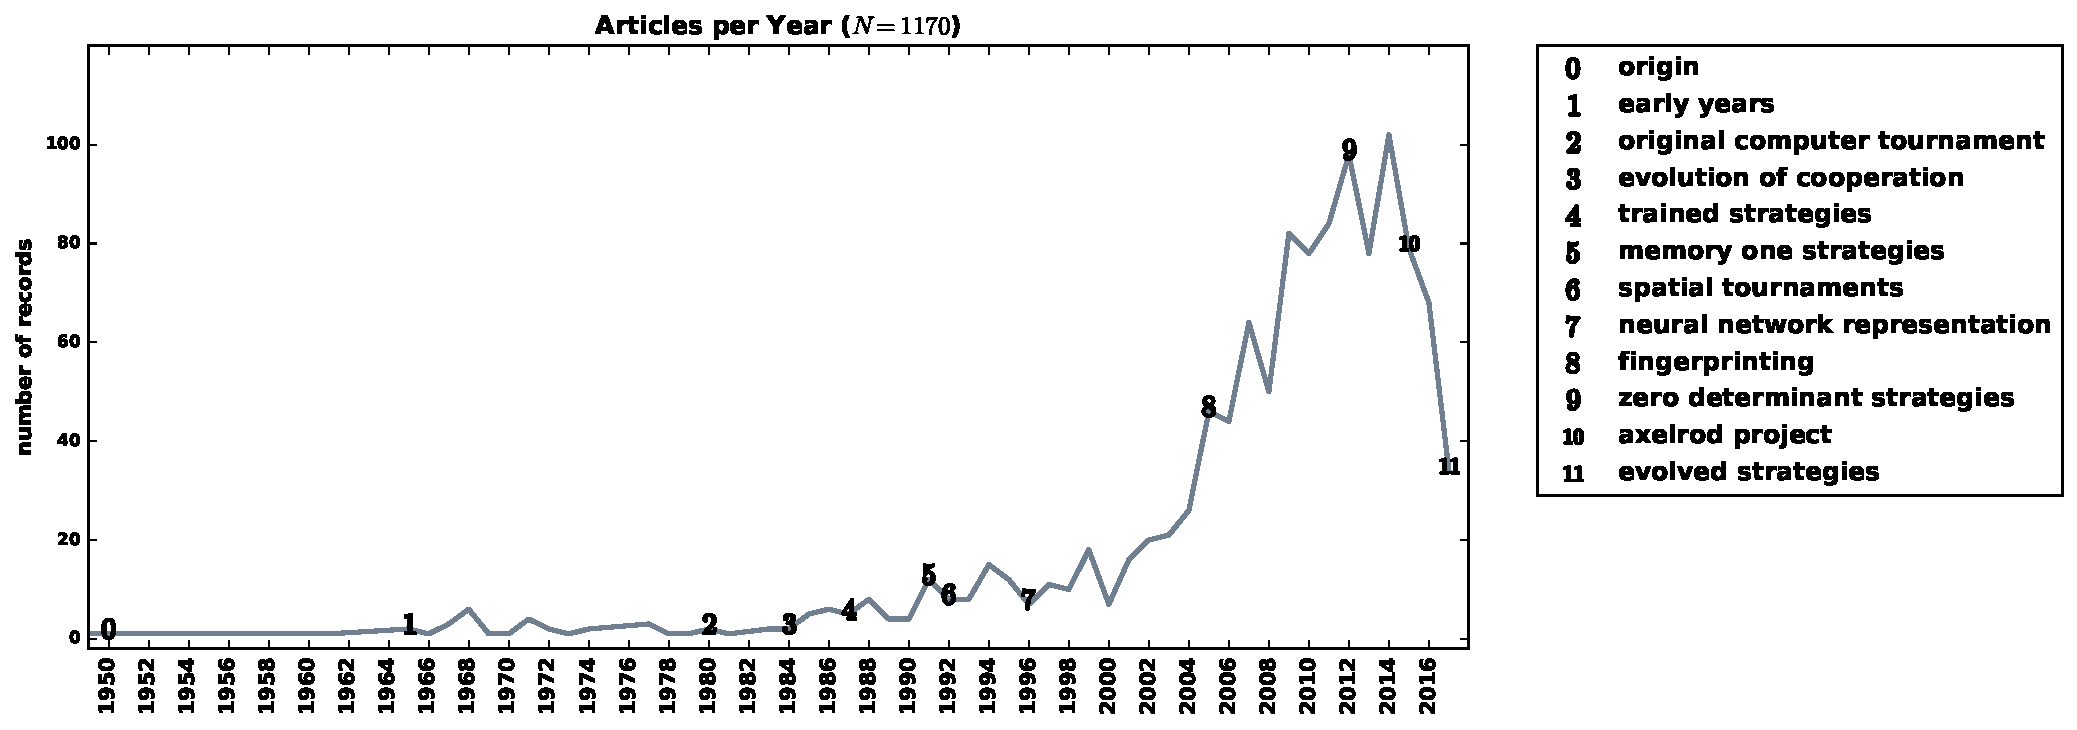
\includegraphics[width=\textwidth]{assets/images/timeline.pdf}
%     \caption{\label{fig:timeline} A timeline of the prisoner's dilemma research.}
% \end{figure}

\section{Timeline}\label{section:timeline}

% \subsection{Origin and Primal research (1961-1972)}

% The origin of the prisoner's dilemma goes back to the 1950s in early experiments
% conducted at the RAND~\cite{Flood1958} to test the applicability of games
% described in~\cite{VonNeumann1944}. Although the name behind the game was given
% later the same year.
% According to~\cite{Tucker1983}, A. W. Tucker (the PhD supervisor of J. Nash),
% in an attempt to delivery the game with a story during a talk used prisoners as
% players and the game has been known as the prisoner's dilemma ever since.

% The study of the prisoner's dilemma has attracted people from various fields
% across the years. An early figure within the field is Prof A. Rapoport,
% a mathematical psychologist, whose work focused on peacekeeping.
% In his early work~\cite{rapoport1965} Rapoport conducted experiments using humans
% to simulate a play of the prisoner's dilemma. Experimental groups have not been
% used only by Rapoport. They are a common mean of studying the game \cite{Evans1966,
% Gallo1968, Lutzker1961, Mack1971, Sensenig1972} used until today. %TODO reference a good article with human studies.

% The early experiments were exploring the conditions under which altruist behaviour emerges
% in human groups. Conditions explored were the gender~\cite{Evans1966,
% Lutzker1961, Mack1971} of individuals, the representation of the game
% \cite{Evans1966}, the distance between players~\cite{Sensenig1972}, the initial effects
% \cite{Tedeschi1968} and whether the experimenter was biased~\cite{Gallo1968}.

% The community however soon came to ask a different question: ``what is the best way to play the game?''
% Inspired by the work of Rapoport a political scientist R. Axelrod conducted the first
% ever, to the author's knowledge, computer tournaments of the IPD. According to
% Axelrod~\cite{Axelrod2012}, he decided to use computers because human participant
% were known to act very randomly even though the aim of the game is clear to them.

% \subsection{Axelrod's Tournaments (1981-1984)}\label{subsection:axelrods_tournament}

% The first computer tournament was performed in 1980~\cite{Axelrod1980a}.
% Several scientists were invited to submit their strategies, written in the
% programming languages Fortran or Basic. There was a total of 13 submissions
% made by the following researchers,

% \begin{multicols}{2}
%     \begin{enumerate}
%         \item T Nicolaus Tideman and Paula Chieruzz;
%         \item Rudy Nydegger;
%         \item Bernard Grofman;
%         \item Martin Shubik;
%         \item Stein and Anatol Rapoport;
%         \item James W Friedman;
%         \item Morton Davis;
%         \item Jim Graaskamp;
%         \item Leslie Downing;
%         \item Scott Feld;
%         \item Johann Joss;
%         \item Gordon Tullock;
%         \item Name not given.
%     \end{enumerate}
% \end{multicols}

% Each competed in a 200 turn match against all 13 opponents, itself and a player
% that played randomly. This type of tournament is referred to as a round robin and
% corresponds to a complete graph from a topological point of view. The tournament
% was repeated \(5\) times to reduce variation in the results. Each participant knew
% the exact length of the matches and had access to the full history of each match.
% Furthermore, Axelrod performed an preliminary tournament and the results were known
% to the participants. The payoff values used for equation(\ref{eq:the_pd_payoffs}) where
% \(R=3, P=1, T=5\) and \(S=0\). These values are commonly used in the literature
% and unless specified will be the values used in the rest of the work described here.

% The winner of the tournament was determined by the total average score and not by
% the number of matches won. The strategy that was announced the winner was
% submitted by Rapoport and was called \textbf{Tit For Tat}. Tit for Tat, is a
% strategy that always cooperates on the first round and then mimics the opponent's
% previous move.

% Examples of Tit for Tat interacting for 8 turns with deterministic opponents are
% given by Tables~\ref{table:tft_vs_c}, \ref{table:tft_vs_d} and \ref{table:tft_vs_a}.
% The opponents are, \textbf{Cooperator} a strategy that always cooperates,
% \textbf{Defector} an opponent that always defects and \textbf{Altenator} a
% player who alternates between cooperating and defecting.

% \begin{table}[!hbtp]
%     \begin{center}
%     \begin{tabular}{lcc}
%         \toprule
%         Turns & Tit for Tat & Cooperator\\
%         \toprule
%         1 & C & C \\
%         2 & C & C \\
%         3 & C & C \\
%         4 & C & C \\
%         5 & C & C \\
%         6 & C & C \\
%         7 & C & C \\
%         8 & C & C \\
%         \bottomrule
%     \end{tabular}
%     \caption{Tit for Tat example match of 8 turns against Cooperator}\label{table:tft_vs_c}
%     \end{center}
% \end{table}

% \begin{table}[!hbtp]
%     \begin{center}
%     \begin{tabular}{lcc}
%         \toprule
%         Turns & Tit for Tat & Defector\\
%         \toprule
%         1 & C & D\\
%         2 & D & D\\
%         3 & D & D\\ 
%         4 & D & D \\
%         5 & D & D\\
%         6 & D & D\\ 
%         7 & D & D \\
%         8 & D & D \\
%         \bottomrule
%     \end{tabular}
%     \caption{Tit for Tat example match of 8 turns against Defector}\label{table:tft_vs_d}
% \end{center}
% \end{table}

% \begin{table}[!hbtp]
%     \begin{center}
%     \begin{tabular}{lcc}
%         \toprule
%         Turns & Tit for Tat & Altenator\\
%         \toprule
%         1 & C & C \\ 
%         2 & C & D \\ 
%         3 & D & C \\ 
%         4 & C & D \\
%         5 & D & C \\ 
%         6 & C & D \\ 
%         7 & D & C \\ 
%         8 & C & D \\
%         \bottomrule
%     \end{tabular}
%     \caption{Tit for Tat example match of 8 turns against Altenator}\label{table:tft_vs_a}
% \end{center}
% \end{table}

% The results of the first tournament were filled with surprises. Tit for Tat the
% simplest strategy of all had won and had managed to defeat even entrants that
% tried to improve on Tit for Tat after the preliminary tournament results.
% Axelrod justified the success of the strategy saying that the strategy was
% `nice' and `forgiving'.

% The top eight ranked strategies were strategies that did no defect on the first
% round, thus they were described as `nice' strategies. Compared to the rest of the
% "nice" strategies, Tit for Tat had also another property. That property was
% `forgiveness'. Tit for Tat punished it's opponent for a defection but just once
% and then it would try to cooperate again. These two properties were described to
% be the secret of success in a prisoner's dilemma tournament.

% In order to further test the robustness of the results Axelrod performed a second
% tournament~\cite{Axelrod1980b} later in 1980. This time a total of 63 participants
% submitted strategies, their names were the following,

% \begin{multicols}{3}
%     \begin{enumerate}
%         \item Gail Grisell;
%         \item Harold Rabbie;
%         \item James W Friedman;
%         \item Abraham Getzler;
%         \item Roger Hotz;
%         \item George Lefevre;
%         \item Nelson Weiderman;
%         \item Tom Almy;
%         \item Robert Adams;
%         \item Herb Weiner;
%         \item Otto Borufsen;
%         \item R D Anderson;
%         \item William Adams;
%         \item Michael F McGurrin;
%         \item Graham J Eatherley;
%         \item Richard Hufford;
%         \item George Hufford;
%         \item Rob Cave;
%         \item Rik Smoody;
%         \item John Willaim Colbert;
%         \item David A Smith;
%         \item Henry Nussbacher;
%         \item William H Robertson;
%         \item Steve Newman;
%         \item Stanley F Quayle;
%         \item Rudy Nydegger;
%         \item Glen Rowsam;
%         \item Leslie Downing;
%         \item Jim Graaskamp and Ken Katzen;
%         \item Danny C Champion;
%         \item Howard R Hollander;
%         \item George Duisman;
%         \item Brian Yamachi;
%         \item Mark F Batell;
%         \item Ray Mikkelson;
%         \item Craig Feathers;
%         \item Fransois Leyvraz;
%         \item Johann Joss;
%         \item Robert Pebly;
%         \item James E Hall;
%         \item Edward C White Jr;
%         \item George Zimmerman;
%         \item Edward Friedland;
%         \item X	Edward Friedland;
%         \item Paul D Harrington;
%         \item David Gladstein;
%         \item Scott Feld;
%         \item Fred Mauk;
%         \item Dennis Ambuehl and Kevin Hickey;
%         \item Robyn M Dawes and Mark Batell;
%         \item Martyn Jones;
%         \item Robert A Leyland;
%         \item Paul E Black;
%         \item T Nicolaus Tideman and Paula Chieruzz;
%         \item Robert B Falk and James M Langsted;
%         \item Bernard Grofman;
%         \item E E H Schurmann;
%         \item Scott Appold;
%         \item Gene Snodgrass;
%         \item John Maynard Smith;
%         \item Jonathan Pinkley;
%         \item Anatol Rapoport.
%     \end{enumerate}
% \end{multicols}

% All the participants knew the results of the previous tournament. The rules
% were similar to those of the first tournament with only one exception;
% the number of turns was not specified instead a fixed probability (refereed to as
% `shadow of the future'~\cite{Axelrod1988}) of the game ending on the next move
% was used. The fixed probability was chosen to be 0.0036 so that the expected
% median length of a match would be 200 turns. The topology was of a round robin
% and each pair of players was matched 5 times. Each of the five matches had a
% length of 63, 77, 151, 308 and 401.

% The first tournament had reported that it paid for a strategy to be nice and forgiving.
% These ideas were carried onto the second tournament from various applicants.
% A total of 39 strategies were now nice and nearly all of them somewhat forgiving.
% There were also two lessons taken from the report of the first tournament:

% \begin{enumerate}
%     \item Be nice and forgiving.
%     \item If others are going to be nice and forgiving take advantage of them.
% \end{enumerate}

% The strategies that based their behaviour on lesson one suffered due to lesson
% two. The strategies following lesson two suffered while trying to exploit their
% opponents. The most successful entries tended to be variants of Tit for Tat,
% such as \textbf{Tit for Two Tats} submitted by John Maynard Smith. Tit for Two
% Tats defects only when the opponent has defected twice in a row. However
% none of the variants managed to outperform the pure version. All that said
% the winner of the second tournament was once again Tit for Tat. The conclusions
% of~\cite{Axelrod1980a} were that the strong performance of the strategy was due to:

% \begin{itemize}
%     \item The strategy would start of by cooperating.
%     \item It would forgive it's opponent after a defection.
%     \item It would always be provoked by a defection no matter the history.
%     \item As soon as the opponents identified that they were playing Tit for Tat,
%     they would choose to cooperate for the rest of the game.
% \end{itemize}
% %The strategies of the second tournament where bias due the first tournament. Discuss with V.
% These characteristics allowed Tit for Tat to achieve the highest average score
% over the 63 rules in the tournament. The repeated success of the strategy soon raised
% a question: Is Tit for Tat the best strategy when playing the iterated prisoner's dilemma? 

% So far it has been discussed how the performance of the strategy has been tested
% through tournaments against other strategies. But is the overall success of a
% strategy based only on it's performance in a round robin tournament or should
% it be checked through other ways as well? R. Axelrod asking the very same question
% performed an `ecological' tournament in 1981~\cite{Axelrod1984}.

% Axelrod argued that some strategies are so unsuccessful that there are very likely
% to be dropped in the future, while other more successful strategies would continue
% in later interactions. Influenced by evolutionary biology Axelrod introduced a way
% of capturing this behaviour, which included running a series of tournaments where
% more successful strategies would occupy a larger part of the environment and the
% less successful strategies would become less often. This is known as an ecological
% tournament.

% The simulation of the process, as described in~\cite{Axelrod1984}, is straightforward.
% Consider matrix~\ref{eq:interaction_payoffs} which provides the expected payoff
% when two individuals of different types interact. Starting with proportions of
% each type in a given generation the proportions of these strategies in the next
% generation is the only measure we need to calculated. This is achieved by
% calculating the weighted average of the scores of a given strategy with all
% other players. The weights are the numbers of the other strategies which
% exist in the current generation. The numbers of a given strategy in the next
% generation is then taken to be proportional to the product of its numbers in the
% current generation and its score in the current generation.

% \begin{equation} \label{eq:interaction_payoffs}
%     \begin{pmatrix}
%     (R=3, R=3) & (S=0, T=5) \\ (T=5, S=0) & (P=1, P=1)
%     \end{pmatrix}
% \end{equation}

% Note that the ecological tournament does not offer any evolutionary perspective.
% There is no possibility of a new strategy to be introduced, there is no mutation
% probability to drive the evolution. The ecological tournament is a framework that provides
% the distributions of given types over time when interacting with the population.

% The set of strategies from Axelrod's second tournament was used to perform the
% ecological tournament. Several interesting insights were reported,

% \begin{itemize}
%     \item The lowest ranking 11 strategies had fallen to half their initial size
%     by the 5 generation;
%     \item The middle-ranking entries managed to hold their initial size;
%     \item By the \(500^{th}\) generation the only strategies that were larger than their
%     initial size have been the top 11 ranked strategies;
%     \item These formed 96\% of the population at that time;
%     \item The rule which ranked fifth in the tournament, submitted by William Adams,
%     grew to three times its original size in the population and then began to sink
%     after generation 100;
%     \item The rule which ranked eighth, submitted by Paul D. Harrington, and was
%     the only non nice rule in the top 15, grew to four times its original size but
%     began to shrink after generation 150 to reach only a third of its original
%     size by the \(1000^{th}\) generation.
% \end{itemize}

% Overall the strategies that did rank at the top of the second tournament have
% also ranked top in the ecological tournament. On the same note, the strategy that
% was ranked at the top was again Tit for Tat. By the 1000th generation it was 14.5\%
% of the whole population, followed by the third place rule at 13.9\% and then the
% second place rule at 13.1\%. Tit for Tat was growing at .05\% per generation which
% was a faster rate than any other strategy. All these are captured by
% Figure~\ref{fig:ecological.tournament}.
% % This is a lie. We said that the table would make more sense here.

% \begin{figure}[!hbtp]
%     \centering
%     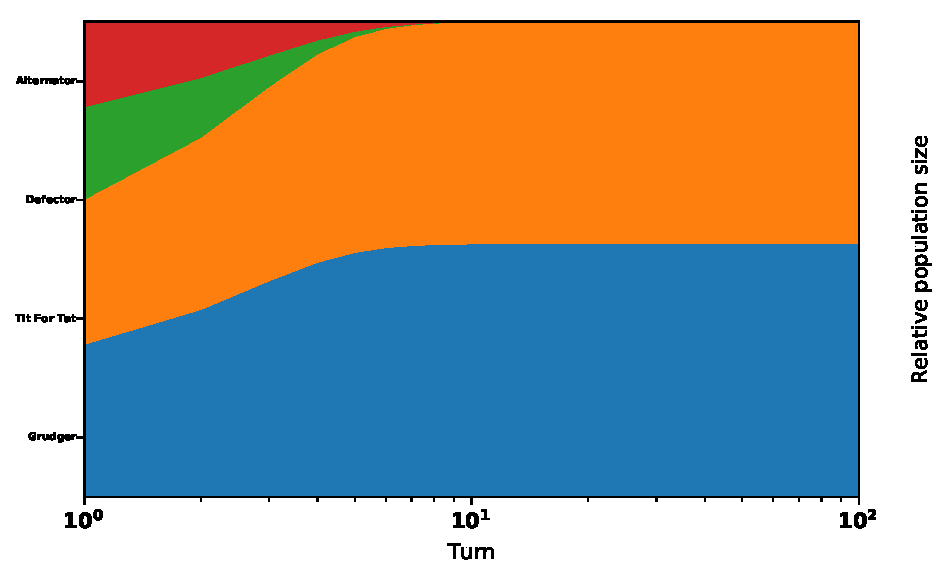
\includegraphics[width=.6\textwidth]{./assets/images/ecological.pdf}
%     \caption{System evolving over time based on natural selection using
%     \cite{axelrodproject}, strategies set from Axelord's second tournament.}
%     \label{fig:ecological.tournament}
% \end{figure}

% A much more general approach was discussed in~\cite{axelrod1981}; the evolutionary
% approach. Imagine a population made up of individuals where everyone follows the
% same strategy, \(B\) and a single individual adopts a mutant strategy \(A\).
% Strategy \(A\) is said to invade strategy \(B\) if,

% \begin{equation}
% V(A \mid B) > V(B \mid B)
% \end{equation}
% where \(V(B \mid B)\) is the expected payoff received by \(B\) against itself.

% Since the strategy \(B\) is an population that interacts only with itself,
% the concept of invasion is equivalent to a single mutant being able to outperform
% the average population. This leads to the concept of the evolutionary approach.
% Thus for a strategy to be \textbf{evolutionary stable} it must be able to
% resists any invasion. There are several applications in biology for the interpretation
% of this approach, for example the survival of the fitness in wildlife.

% The ability of strategies to be favoured under natural selection and their
% ability to withstand invasion from other strategies soon became a measure
% of performance; refereed to as the stability of a strategy.

% Due the large number of possible strategies in the prisoner's dilemma identifying
% all the stable strategies was a difficulty task at the time. Axelrod focused
% the work of~\cite{axelrod1981} in three questions,

% \begin{enumerate}
%     \item Under what conditions was Tit for Tat evolutionary stable?
%     \item What were the necessary and sufficient conditions for any strategy to be
%     evolutionary stable?
%     \item Finally, in an environment where all followed a strategy of unconditional
%     defection, can cooperation emerge?
% \end{enumerate}

% A series of theorems were presented which showed, that Tit for Tat is evolutionary
% stable if and only if it is invadable neither by Defector nor Alternator. This
% is true only if the game is likely to last long enough for the retaliation
% to counteract the temptation to defect, according to Axelrod. Secondly,
% Defectors can withstand invasion by any strategy, as long as the players using
% other strategies come one at a time. But if they come in clusters (even in rather small
% clusters), the strategy could be invaded. As for the characteristics of stable
% strategies, Axelrod provided a series of theorems.

% Overall, all of Axelrod's tournaments offered many insights and new concepts to the field.
% These were not only limited on Tit for Tat. For example several strategies of
% these tournaments are still being used in literature to date, such as Tit for
% Two Tats and \textbf{Grudger}.

% Grudger was originally submitted by James W. Friedman. Grudger is a strategy that
% will cooperate as long as the opponent does not defect. The name Grudger was give
% to the strategy in~\cite{Li2014}. Though the strategy goes by many names in the
% literature such as, Spite~\cite{Beaufils1997}, Grim Trigger~\cite{Banks1990} and
% Grim~\cite{Van2015}.

% Though not all strategies of Axelrod's tournament are retrievable. The author
% had given a explanation of all 13 strategies of the first tournament.
% The size of the second tournament did not allow him this time to go into details
% for every single participant. The author mainly focused on the high ranked participants.
% However, the source code of the 63 strategies can be found on Axelrod's personal
% website~\cite{fortan_code}. Figure~\ref{fig:tit_for_tat_fortran} serves as an
% example of the source code for the winning strategy Tit for Tat.

% \begin{figure}[!hbtp]
%     \centering
%     \begin{minted}
%         [
%         autogobble=true,
%         framesep=2mm,
%         fontsize=\normalsize,
%         ]
%         {fortran}
%     FUNCTION K92R(J,M,K,L,R, JA)
% C BY ANATOL RAPOPORT
% C TYPED BY AX 3/27/79 (SAME AS ROUND ONE TIT FOR TAT)
% c replaced by actual code, Ax 7/27/93
% c  T=0
% c   K92R=ITFTR(J,M,K,L,T,R)
%       k92r=0
%       k92r = j
% c test 7/30
% c   write(6,77) j, k92r
% c77   format(' test k92r. j,k92r: ', 2i3)
%       RETURN
%       END
%     \end{minted}
%     \caption{\label{fig:tit_for_tat_fortran} Source code for Tit for Tat in Fortran.
%     Provided by~\cite{fortan_code}.}
% \end{figure}

% Note though that the code of the second tournament only includes the strategies.
% The code for running a round robin tournament or an ecological tournament
% is not given. Moreover, the source code of the first 13 strategies is not
% available, as stated in Axelrod's personal website~\cite{fortan_code}.

% \subsection{Response to the computer tournaments (1984-1993)}
% \label{section:responses_to_computer_tournament}

% The pioneering work of computer tournaments and the results of the reciprocal behaviour
% in the prisoner's dilemma spread the knowledge of the game worldwide and across
% disciplines. Several researchers responded immediately to Axelrod's tournaments
% and the study of cooperation became of critical interest once again.
% This section focuses on the research that was carried out after the initial
% computer tournaments. More specifically the research the falls in the following
% categories, over the time period between 1984 and 1993, are considered in this section:

% \begin{itemize}
%     \item Applications of the iterated prisoner's dilemma, the famous strategy
%     Tit for Tat and the reciprocal behaviour.
%     \item Computer tournaments under stochastic uncertainty and the introduction
%     of new strategies.
% \end{itemize}

% One of the scientific disciplines that immediately employed Axelrod's work has
% been the ecological field. More specifically, the works of~\cite{Craig1984,
% Dugatkin1988, Godfray1992, Milinski1987, Wilkinson1984}.
% In~\cite{Dugatkin1988, Milinski1987} the behaviour of fish when confronting a
% potential predator was studied. Conflicts can arise within pairs of fish in these
% circumstances. In both works experiments were held using a system of mirrors
% where sticklebacks and guppies respectively, would be accompanied by a cooperating
% companion or a defecting one. In both cases the hypothesis that the fish would
% behave according to Tit for Tat and that cooperation would evolve was supported.
% The works of~\cite{Godfray1992, Wilkinson1984} looked at food sharing between
% vampire bats and explained behaviour based on known strategies.

% Another quick response to the tournaments was that of~\cite{Molander1985}.
% It was argued that Axelrod's work assumed that each player had a perfect
% information of the opponent's actions. In real life situations this is not always
% the case. Interactions often suffer from measures of uncertainty and this was not
% captured in the original tournaments. Molander studied the performance of Tit for
% Tat in an uncertain environment by introducing noise. A probability that a player's
% move will be flipped. It was proven that when two strategies playing Tit for Tat
% met in a noisy match the average payoff of each strategy would be the same as
% that of a Random player (with a probability \(0.5\) of cooperating).

% In 1988 publications from other disciplines were using the iterated prisoner's
% dilemma and Axelrod's work for teaching and social studies.
% In~\cite{Levitt1988} a version of the prisoner's dilemma which set the
% problem in an ordinary business context was used as a pedagogic instrument within
% graduate business students. The work of~\cite{Rabow1988} considered non zero sum
% games, specifically the prisoner's dilemma, and illustrated the impact they
% have on societal problems such as war.

% In 1989 reactive strategies are introduced in~\cite{nowak1989}. Reactive strategies
% are a set of players that take into account only the last move of the opponent. 
% Thus, they can be represented by the probability of cooperating after an opponent's
% \textbf{C} or \textbf{D}. The same author a year later in 1990 gave a formal
% definition of a memory one~\cite{Nowak1990}. Memory one strategies consider the
% entire history of the previous turn to make a decision. Thus reactive strategies are
% a subset of memory one.

% If only a single turn of the game is taken into account and depending on the
% simultaneous moves of two players there are only four possible states that
% players could possibly be in. These are \(CC, CD, DC\) and \(DD\). A memory one
% strategy is denoted by the probabilities of cooperating after each of these states,
% \( p = (p_1, p_2, p_3, p_4) \in\mathbb{R}_{[0,1]}^{4} \).
% A match between two memory one players \(p\) and \(q\) can be modelled as a
% stochastic process, where the players move from state to state. More specifically,
% it can be modelled by the use of a Markov chain, which is described by a matrix 
% \(M\).

% \begin{equation}\label{eq:markov_matrix}
%     M =
% \begin{bmatrix}
%     p_{1} q_{1} & p_{1} (- q_{1} + 1) & q_{1} (- p_{1} + 1) & (- p_{1} + 1) (- q_{1} + 1)
%     \\
%     p_{2} q_{3} & p_{2} (- q_{3} + 1) & q_{3} (- p_{2} + 1) & (- p_{2} + 1) (- q_{3} + 1)
%     \\
%     p_{3} q_{2} & p_{3} (- q_{2} + 1) & q_{2} (- p_{3} + 1) & (- p_{3} + 1) (- q_{2} + 1)
%     \\
%     p_{4} q_{4} & p_{4} (- q_{4} + 1) & q_{4} (- p_{4} + 1) & (- p_{4} + 1) (- q_{4} + 1)
%     \\
% \end{bmatrix}
% \end{equation}

% The players are assumed to move from each state until the system reaches a state
% steady.  The utility of a player can be given by multiplying the steady states of
% \(M\) by the payoffs of equation(\ref{eq:the_pd_payoffs}). Thus~\cite{Nowak1990}
% offered a mathematical framework to calculate the utility of two players without
% simulating the game. Memory one strategies are considered an important family of
% strategies and the formulation given in 1990 is still being used to date.

% A player called \textbf{Handshake} was presented by~\cite{Robson1989} in 1989.
% Handshake is a strategy that starts with cooperation, defection. If the opponent
% plays in a similar way then it will cooperate forever, otherwise it will defect
% forever. Handshake has a property that will be revisited in this literature
% review which is it's recognition property.

% From 1991 to 1992, further research explored the performance of Tit for Tat in uncertain
% environments. These works include~\cite{Godfray1992, Bendor1991, Nowak1992}.
% In~\cite{Bendor1991} a similar tournament to that of Axelrod's was performed,
% but this time it was a noise tournament. Bendor had invited researchers from several
% departments across his university and from a university seminar. Each match
% would last a random number of turns, with a probability of 0.0067 of ending in
% the next turn. The probability of noise was a random variable, distributed normally
% with a mean of zero and a standard deviation of eight. The results of his
% tournament demonstrated that Tit for Tat performed rather poorly and the highest
% ranked strategies were generous ones. The top ranked strategy was \textbf{Nice and Forgiving}.

% The work of~\cite{Nowak1992} aimed to also investigate stochastic effects.
% This is was done using an evolutionary setting of a heterogeneous population
% with noise. The author investigate which strategies would manage to take over
% the population and would be evolutionary stable. The strategies were explored
% over the space of reactive strategies. The results demonstrated that 
% though a small fraction of Tit for Tat players have been essential for the emergence
% of cooperation, more generous strategies took over the population. More specifically
% the re active strategy known as \textbf{Generous Tit for Tat} which is presented as
% \((0, \frac{2}{3})\).

% The author of~\cite{Nowak1992, nowak1989, Nowak1990} also introduced another
% important strategy of the literature. It was presented in~\cite{Nowak1993} and
% is it known as \textbf{Pavlov}. Pavlov is a strategy with the tolerance of Generous Tit for Tat
% but also the capability of resisting and invading an all-out cooperators population.
% The strategy is based on the fundamental behavioural mechanism win-stay,
% lose-shift. It starts off with a cooperation and then repeats it's previous move
% only if it was awarder with a payoff of \(R\) or \(T\). Otherwise it shifts
% it's last move.
 
% \subsection{Evolutionary Dynamics (1987-1999)}
% % This needs work I know
% Determining the evolutionary stability of strategies for the iterated prisoner's
% dilemma as we discussed is not an easy task. Methods can be use to deal with
% the difficulty. In~\cite{Boyd1987} the author restricted the possible strategies
% that could be adopted to a relatively narrow set and resulted that no pure strategy
% is evolutionary stable, including Tit for Tat. Arguing with the results presented
% in~\cite{axelrod1981}. The list of strategies used included strategies such as
% Defector and \textbf{Suspicious Tit for Tat}, a strategy that plays
% Tit for Tat but starts by defecting.

% The results were questioned by~\cite{May1987}, stating that much was still no fully
% explored and more research had to be put into the results. Farrel and Ware in
% 1989~\cite{Farrell1989} extended the result to include finite mixture of pure
% and mixtures of Tit For \(n\) Tats as well. On the same year the work of~\cite{Boyd1989}
% looking again at a narrow set of strategies extended their results to
% noisy environments.

% Evolutionary dynamics have been highly useful in the research of the prisoner's
% dilemma. In~\cite{Axelrod1987}, an evolutionary process, called the genetic
% algorithm, was used to discover effective strategies. The author introduced
% lookup tables as a mean of representing a strategy in a gene format. A lookup
% table is a set of deterministic responses based on the opponents \(m\) last
% moves; \cite{Axelrod1987} considered \(m=3\).

% An extension to the natural selection was introduced in the 1992~\cite{Nowak1992b},
% recommending a different type of topology. A population of two deterministic
% strategies, Defector and Cooperator, were placed on a a two dimensional square array
% where the individuals could interact only with the immediate neighbours.
% The number of immediate neighbours could be either, fourth, six or eight. As
% shown in Figure~\ref{fig:topologies}. The authors claimed that the essential
% results remain true of all topologies; the results also hold whether self interactions
% are taken into account.

% Thus each cell of the lattice is occupied by a Cooperator or a Defector. At
% each generation step each cell owner interacts with its immediate neighbours.
% The score of each player is calculated as the sum of all the scores the player
% achieved at each generation. At the start of the next generation, each lattice
% cell is occupied by the player with the highest score among the previous owner
% and the immediate neighbours. This topology is refereed to as spatial topology.

% Nowak studied the population dynamics as a function of the temptation payoff.
% It was shown that for different values of the temptation payoff, cooperators
% and defectors could persist together.

% \begin{figure}[!hbtp]
% \centering
%     \begin{subfigure}{.25\textwidth}
%         \hspace{.8cm}
%         \includestandalone[width=0.6\textwidth]{assets/tex/neighb_four}
%     \end{subfigure}
%     \begin{subfigure}{.25\textwidth}\centering
%         \includestandalone[width=0.6\textwidth]{assets/tex/neighb_eight}
%      \end{subfigure}
%      \begin{subfigure}{.25\textwidth}\centering
%         \includestandalone[width=0.6\textwidth]{assets/tex/neighb_six}
%      \end{subfigure}
%     \begin{subfigure}{.25\textwidth}
%         \includestandalone[width=\textwidth]{assets/tex/square_lattice}
%     \end{subfigure}
%     \begin{subfigure}{.25\textwidth}\centering
%         \includestandalone[width=\textwidth]{assets/tex/square_lattice_eight}
%      \end{subfigure}
%      \begin{subfigure}{.25\textwidth}\centering
%         \includestandalone[width=\textwidth]{assets/tex/hexagonal_lattice}
%      \end{subfigure}
%      \caption{Spatial neighbourhoods}\label{fig:topologies}
%     \end{figure}

% This work dealt with dealt with symmetric spatial lattices in two dimensions,
% deterministic winning and discrete time. The authors in later work~\cite{nowak1994},
% that the results remain valid in more realistic situations. Such as situations
% where the spatial distributions of cells are random in two or three dimensions,
% and where winning is partly probabilistic.

% \subsection{Modern approaches (1995-2015)}\label{section:modern_approaches}

% In this section we will cover several research projects published between 1995
% and 2015. The research reviewed here focuses on computer tournaments and serves
% as an introduction to various strategies that have made an impact in the literature.

% Initially in 1995 a combination of tournament studies, ecological simulations
% and theoretical analysis was used in~\cite{Wu1995} to demonstrate approaches on
% coping with noise. The first approach was \textit{generosity}. A more generous version
% of Tit for Tat, the strategy called the Generous Tit for Tat, was proven to be
% highly effective against players that were not adapted to noise. The second
% approach introduced was \textit{contrition}. The authors stated that when
% interacting with strategies that have been adapted to noise a contrite version 
% of Tit for Tat is even more effective at quickly restoring mutual cooperation 
% without the risk of exploitation. The strategy introduced as the contrite variant
% was called \textbf{Contrite Tit for Tat}. A strategy which three states:
% \textit{contrite, content, provoked}. It begins by cooperating and stays there unless
% there is a unilateral defection. If it was the victim of a defection while content
% the strategy becomes provoked and defects until the opponent cooperates, and 
% causes it to become content. If it was the defector while content, it
% becomes contrite and cooperates. When contrite it becomes content only after
% there has been a mutual cooperation. The final approach has been using strategy
% Pavlov. Moreover, in the analysis an variant of Pavlov was also included
% called Generous Pavlov, a variant that cooperates 10\% of the times when it 
% would either wise had defected. Though all approaches were effecting in coping
% with noise in a standard tournament, the authors argued that Pavlov was not 
% suited for ecological tournaments.

% An interesting approach of to capture promising strategies for the game
% was written in 1996 by~\cite{Miller1996}. Strategies represented by finite automata
% were learning to update their choices through an explicit evolutionary process
% modelled by a genetic algorithm.

% Strategies based on finite state machines are described by the number of states.
% The strategy selects the next action in each round based on the current state
% and the opponent's last move, transitioning to a new state each time.
% Figure~\ref{fig:tit_for_tat_fsm}, illustrates the finite state representation
% of Tit For Tat.

% \begin{figure}[!hbtp]
%     \centering
%     \includestandalone[width=.3\textwidth]{./assets/tex/tit_for_tat_fsm}
%     \caption{Finite state machine representation of Tit for Tat.}
%     \label{fig:tit_for_tat_fsm}
% \end{figure}

% In 1997, \textbf{Gradual} a well performed strategy and a commonly known in the
% literature was proposed by~\cite{Beaufils1997}. Gradual starts off by cooperating,
% then after the first defection of the other player, it defects one time and cooperates
% twice. After the second defection of the opponent, it defects two times and cooperates
% twice. After the \(n^{th}\) defection it reacts with \(n\) consecutive defections 
% and then two cooperations. Gradual had managed to outperform strategies such
% as Tit for Tat and Pavlov.

% Though several of this tournament discussed so far were generated using computer
% code not all of the source code was made available by the authors. Several
% open projects were created and published through the year. The first one
% discussed in this work, excluding the code for Axelrod's strategies, is 
% PRISON~\cite{prison}. PRISON is written in the programming language Java and
% preliminary version was launched on 1998. It was used by it's authors in several
% publications. The project includes a good number of strategies from the
% literature but unfortunately the last update of the project dates back in 2004.

% Another measure of uncertainty discussed in 1998~\cite{Hoffmann1998} is that of
% mis perception. Mis perception is the probability that the opponent's current
% move is flipped before being recorded to the history. Results of~\cite{Hoffmann1998}
% indicated that noise effected the emergence of cooperative behaviour in the
% populations. In 1999, \cite{Turner1999} uses evolutionary game theory to study
% the spread of virus.

% Following the success of Gradual the authors of~\cite{tzafestas-2000a}
% conducted a tournament of 13 strategies just to outperform it. Their strategy
% was the \textbf{Adaptive Tit for Tat} and the algorithm used by it is given by
% \ref{alg:adaptive_tft}.

% \begin{algorithm}
% \begin{algorithmic}[1]
%     \IF{opponent played \textbf{C} in the last cycle}
%      \STATE world = world + \(r(1-\text{world})\), \(r\) is the adaptation rate
%     \ELSE
%      \STATE work = world + \(r(0 - \text{world})\)
%      \ENDIF
%     \IF{world \(\geq\) 0.5}
%         \STATE play \textbf{C}
%     \ELSE
%     \STATE play \textbf{D}
%     \ENDIF
% \end{algorithmic}
% \caption{Adaptive Tit for Tat.}
% \label{alg:adaptive_tft}
% \end{algorithm}

% Adaptive Tit for Tat ranked first in it's tournament surpassing Gradual. However,
% the results were drawn from a tournament of 13 strategies.

% % Less generous variants also made an appearance~\cite{Hilde2013}.
% % \textbf{Anti Tit for Tat}, is a strategy that plays the opposite of the opponents
% % previous move. Another limitation of the strategy was discussed in~\cite{Wolfgang2006}.
% % Tit for Tat was proven to hit a loop between cooperation and defection.
% % \textbf{Omega Tit For Tat} was introduced and was a strategy capable of avoiding
% % such problem~\cite{Wolfgang2006}.

% In~\cite{Ashlock2006b} the author presented two new strategies that have
% been trained using a finite state machine representation. They are called,
% \textbf{Fortress3} and \textbf{Fortress4}. Figure~\ref{fig:fortress3_and_4}
% illustrates their diagrammatic representation where the transition arrows are
% labelled \textit{O/P} where \textit{O} is the opponent's last action and \textit{P}
% is the player's response.

% \begin{figure}[!hbtp]
% \centering
%     \begin{subfigure}{.4\textwidth}
%         \includestandalone[width=\textwidth]{assets/tex/fortress_3}
%     \end{subfigure}
%     \begin{subfigure}{.4\textwidth}\centering
%         \includestandalone[width=\textwidth]{assets/tex/fortress_4}
%      \end{subfigure}
%      \caption{Representations of Fortress 3 and Fortress 4. Note that the
%      strategy's first move, enters state 1, is defection for both strategies.}
%      \label{fig:fortress3_and_4}
% \end{figure}

% Optimisation methods return a spectrum of strategies. In order to distinguish
% the strategies and assuring that they are indeed different~\cite{Ashlock2005}
% introduced a method called fingerprinting.

% The method of fingerprinting is a technique for generating a functional signature for a
% strategy~\cite{Ashlock2008}. This is achieved by computing the score of a strategy
% against a spectrum of opponents. The basic method is to play the strategy
% against a probe strategy with varying noise parameters. In~\cite{Ashlock2005}
% Tit for Tat is used as the probe strategy. Fingerprint functions
% can then be compared to allow for easier identification of similar strategies.
% In Figure~\ref{fig:fingerprinting} an example of Pavlov's fingerprint is given.
% Fingerprinting has been studied in depth in~\cite{Ashlock2008, Ashlock2009,
% Ashlock2010, Ashlock2006a}.

% \begin{figure}[!hbtp]
%     \centering
%     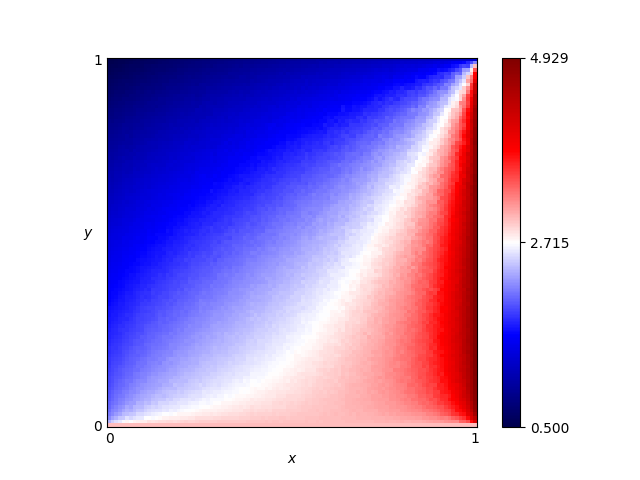
\includegraphics[height=.3\textheight]{./assets/images/Win-Stay_Lose-Shift.png}
%     \caption{Pavlov fingerprinting with Tit for Tat used as the probe strategy.
%     Figure was generated using~\cite{axelrodproject}.}
%     \label{fig:fingerprinting}
% \end{figure}

% The adaptive behaviour that was tried to be capture by~\cite{tzafestas-2000a}
% was not constrained only on Tit for Tat. In~\cite{Li2011} \textbf{APavlov},
% which stands for adaptive Pavlov, made an appearance.  The strategy attempts to
% classify the opponent as one of the following strategies, All Cooperator,
% All Defector, Pavlov, Random or \textbf{PavlovD}. PavlovD, is just Pavlov
% but it starts the game with a \textbf{D}. Once Adaptive Pavlov has classified
% the opponent plays to maximize it's payoff.

% In 2011 the authors of~\cite{Li2011} performed their own tournament where
% several interesting strategies made an appearance.

% \begin{itemize}
%     \item \textbf{Periodic player CCD}, plays \textbf{C}, \textbf{C}, \textbf{D}
%     periodically. Note that variations of a period player also make appearance
%     in the article but will not be listed here.
%     \item \textbf{Prober}, starts with the pattern \textbf{D}, \textbf{C}, \textbf{C}
%      and then defects if the opponent has cooperated in the second and third move;
%      otherwise, it play as Tit for Tat.
%     \item \textbf{Reverse Pavlov}, a strategy that does the reverse of Pavlov.
% \end{itemize}

% \subsection{Zero determinant (2012 - 2015)}

% In 2012 Press and Dyson~\cite{Press2012} studied the iterated prisoner's dilemma and presented
% a new set of strategies called \textbf{zero determinant (ZD)}. The ZD strategies
% are memory one strategies that manage to force a linear relationship between their
% score and that of the opponent.

% In Section~\ref{section:responses_to_computer_tournament} it was described how
% the payoffs of two players could be retrieved by formulating their interactions
% using a Markov chain. Let us denote the payoffs of players \(p\) and \(q\) as:

% \begin{align*}
%     s_p = v S_p \\
%     s_q = v S_q
% \end{align*}

% where \(v\) is a vector of the steady states of matrix \(M\) and \(S_p\), \(S_q\)
% are the equivalent payoff values of the players for each state \(CC, CD, DC, DD\).
% Using linear algebra, Press and Dyson showed that the dot product of the stationary
% distribution of \(v\) with any vector \(f\) can be expressed as a \(4\times 4\)
% determinant. In which one column is \(f\), one column is entirely under the control
% of player \(p\) and another column is entirely under the control of player \(q\).

% This meant that either \(p\) or \(q\) could independently force the dot product
% of \(v\) with some other chosen vector \(f\) to be zero by choosing their
% strategy so as to make the column they control be proportional to \(f\).
% In particular, by \( f = \alpha S_p + \beta S_q + \gamma\), any player can force
% a given linear relation to hold between the long-run scores of both players.

% Press and Dyson's results suggested that the best strategies were selfish ones
% that led to extortion, not cooperation. Arguing with Axelrod's reports.
% All the more, their work stated that in the iterated prisoner's dilemma, memory
% is not advantageous.

% The ZD strategies have attracted a lot of attention. It was stated that
% ``Press and Dyson have fundamentally changed the viewpoint on the Prisoner's
% Dilemma''~\cite{Stewart2012}. In~\cite{Stewart2012}, they ran a variant of
% Axelrod's tournament with 19 strategies to test the effectiveness of 
% ZD strategies. While conducting their tournament they have implement several
% strategies discussed by~\cite{Press2012} and revealed a set of generous ZDs
% the~\textbf{Generous ZD}.

% In~\cite{Lee2015}, the `memory of a strategy does not matter' statement was
% questioned. A set of more complex strategies, strategies that take in account
% the entire history set of the game, were trained and proven to be more stable than
% ZD strategies.

% % Include Moran paper.

% \subsection{Contemporary period (2015 - 2017)}

% In the following section we report research and publications from 2015 to 2017.
% It will focus on sophisticated strategies and computer software.

% In 2015, an open source library, called the Axelrod project~\cite{axelrodproject}
% was launched. The project is written in the programming language
% Python, it is accessible and open source. To date the list of strategies implemented
% within the library exceed the 200. The project has been used in several
% publications including~\cite{Knight2017} and a paper describing it and
% it's capabilities was published in 2016~\cite{Knight2016}. The source code
% for Tit for Tat as implement within the library is shown in Figure
% \ref{fig:tit_for_tat_axelrod}. Furthermore, performing a tournament
% with a selection of strategies is possible in five lines of code, shown in
% Figure~\ref{fig:tournament_code}.

% \begin{figure}[!hbtp]
%     \centering
%     \begin{minted}
%         [
%         autogobble=true,
%         framesep=2mm,
%         fontsize=\normalsize,
%         ]
%         {python}
% def strategy(self, opponent: Player) -> Action:
%     """This is the actual strategy"""
%     # First move
%     if not self.history:
%         return C
%     # React to the opponent's last move
%     if opponent.history[-1] == D:
%         return D
%     return C
%     \end{minted}
%     \caption{\label{fig:tit_for_tat_axelrod} Source code for Tit for Tat in Python
%     as implemented in Axelrod Python library~\cite{axelrodproject}}.
% \end{figure}

% \begin{figure}[!hbtp]
%     \centering
%     \begin{minted}
%         [
%         autogobble=true,
%         framesep=2mm,
%         fontsize=\normalsize,
%         ]
%         {python}
% >>> import axelrod as axl
% >>> players = (axl.Cooperator(), axl.Defector(), axl.TitForTat(), axl.Grudger())
% >>> tournament = axl.Tournament(players)
% >>> results = tournament.play()
% >>> results.ranked_names
% ['Defector', 'Tit For Tat', 'Grudger', 'Cooperator']
%     \end{minted}
%     \caption{\label{fig:tournament_code} Performing a computer tournament
%     using~\cite{axelrodproject}.}
% \end{figure}

% In~\cite{Rapoport2015}, the authors claim that they have managed to
% re-run the first tournament that Axelrod performed. They tried to push his work
% further by altering aspects such as, the format of the tournament, the objective
% and the population. One of the authors claimed to have been a contributor
% to the first tournaments, which would explain how it was managed to reproduce
% the tournament.

% A number of strategies based on artificial neural networks are
% introduced by~\cite{Knight2017}, in 2017. Artificial neural networks provide a mapping
% function to an action based on a selection of features computed from the history
% of play.

% These strategies are refereed to as \textbf{EvovlvedANN} strategies and are
% based on a pre-trained neural network with the following features,

% \begin{multicols}{2}
%     \begin{itemize}
%         \item Opponent's first move is C
%         \item Opponent's first move is D
%         \item Opponent's second move is C
%         \item Opponent's second move is D
%         \item Player's previous move is C
%         \item Player's previous move is D
%         \item Player's second previous move is C
%         \item Player's second previous move is D
%         \item Opponent's previous move is C
%         \item Opponent's previous move is D
%         \item Opponent's second previous move is C
%         \item Opponent's second previous move is D
%         \item Total opponent cooperations
%         \item Total opponent defections
%         \item Total player cooperations
%         \item Total player defections
%         \item Round number
%     \end{itemize}
% \end{multicols}

% A representation of \textbf{EvovlvedANN 5} is given in Figure~\ref{fig:ann_5_neural}.
% The inputs of the neural network are the 17 features as listed above. Number 5
% reefers to the size of the hidden layer.

% \begin{figure}[!hbtp]
%     \centering
%     \includestandalone[width=.5\textwidth]{./assets/tex/ann_5_neural}
%     \caption{Neural network representation of EvovlvedANN 5.}
%     \label{fig:ann_5_neural}
% \end{figure}

% In~\cite{Knight2017}, these representing methods are refereed to as archetypes.
% Finite state machines and artificial neural networks are included in the
% work but also new archetypes are introduced, such as hidden Markov models. A variant
% of a finite state machine that use probabilistic transitions based on the prior
% round of play to other states and cooperate or defect with various probabilities
% at each state. Finite state machines and hidden Markov models
% based strategies are characterized
% by the number of states. Similarly, artificial neural networks based players
% are characterized by the size of the hidden layer and number of input features.

% Additionally a variant of a look up table is also presented called the lookerup
% archetype. The lookerup archetype responses based on the opponent's first \(n_1\)
% moves, the opponent's last \(m_1\) moves, and the players last \(m_2\) moves.
% Taking into account the initial move of the opponent can give many insights.
% For it is the only move a strategy is truly itself without being affected by
% the other player. As a reminder, Axelrod in his work
% highlighted the importance of the initial move and believed that it was one
% of the secrets of success of the strategy Tit for Tat. Finally, a new archetype
% called the Gambler is also introduced, which is a
% stochastic variant of the lookerup archetype.

% In~\cite{Knight2017} evolutionary algorithms are used to introduce as stated
% by the authors the best performing strategies for the iterated prisoner's dilemma.
% These strategies will be refereed  as \textbf{Evolved} strategies.
% Several successful new strategies are,

% \begin{itemize}
%     \item \textbf{EvolvedLookerUp2\_2\_2} a looker up strategy trained with a
%     genetic algorithm; EvolvedLookerUp2\_2\_2 responses based on the opponent's
%     2 first and last moves and the player's 2 last moves. Thus \(n_1=2, m_1=2\)
%     and \(m_2=2\).
%     \item \textbf{Evolved HMM 5} a 5 states hidden markov model trained with a genetic
%     algorithm;
%     \item \textbf{Evolved FSM 16} a 16 state machine trained with a genetic
%     algorithm;
%     \item Finally \textbf{PSO Gambler 2 2 2} a looker up strategy trained with
%     a particle swarm algorithm, where \(n_1=2, m_1=2\) and \(m_2=2\).
% \end{itemize}

% Though several papers have claimed before to have discovered the dominant
% strategies for the game the work of \cite{Knight2017} is promising.
% This is due the fact that the introduced strategies have been trained using
% different types of evolutionary algorithms in a pool of 176 well known
% strategies for the literature. Including all the strategies that have been
% discussed in this section.

% Other recent software projects include~\cite{pd_trust, pd_game}, both are education
% platforms and not research tools. In~\cite{pd_trust}, several concepts such as
% the iterated game, computer tournaments and evolutionary dynamics are introduced
% through a user interface game. Project~\cite{pd_game} offers a big collection of
% strategies and allows the user to try several match and tournaments configurations.
% Such as noise.

\section{Analysing a large corpus of articles}\label{section:analysis}

The focus of the paper is the academic publications on the topic the iterated
prisoner's dilemma. Whilst in Section~\ref{section:timeline} we covered
several publication of specific interest and manually partitioned the literature
in different sections, in the second part of this paper we analyse the publications
using a large dataset of articles. The data collection process is covered in
Section~\ref{section:data_collection} and a preliminary analysis of the data is
conducted in Section~\ref{section:preliminary_analysis}. In Section~\ref{section:methodology},
the methodology on analysing the authors relationships is discussed. This is done
using graph theoretical methods to ascertain the level of collaborative nature
of the field and identify influence, relative to:

\begin{itemize}
    \item Two other sub fields of game theory: auction games~\cite{menezes2005} and 
    the price of anarchy~\cite{roughgarden2005}.
    \item A temporal analysis.
\end{itemize}

Finally in Section~\ref{section:results}, the results of the analysis are presented.

\subsection{Data Collection}\label{section:data_collection}

Academic articles are accessible through scholarly databases and collections of
academic journals. Several databases and collections today offer access through
an open application protocol interface (API). An API allows users to query
directly a journal's database and bypass the user interface side of the journal.
Interacting with an API has two phases: requesting and receiving.
The request phase includes composing a url with the details of what is wanted. For
example, \url{http://export.arxiv.org/api/query?search_query=abs:prisoner's dilemma&max_results=1}
represents a request message. The first part of the request is the address
of the API we are querying.

In this example the address corresponds to the API of arXiv.
The second part of the request contains the search arguments. In our example we
are requesting for a single article that the word `prisoners dilemma' exists within
it's title. The format of the request message is different from API to API.
The receive phase includes receiving a number of raw metadata of articles that
satisfied the request message. The raw metadata are commonly received in extensive markup
language (xml) or Javascript object notation (json) formats~\cite{nurseitov2009}.
Similarly to the request message, the structure of the received data differs from journal
to journal.

The data collection is crucial to this study. To ensure that this study can be
reproduced all code used to query the different APIs has been packaged as a Python library and is
available online~\cite{nikoleta_2017}. The software could be used for any type of
projects similar to the one described here, documentation for it is available at:
\url{http://arcas.readthedocs.io/en/latest/}.
Project~\cite{nikoleta_2017} allow us to collect articles from a list of APIs by
specifying just a single keyword. Four prominent journal in the field and a
pre print server were used as sources to collect data for this analysis. Those
were PLOS, Nature, IEEE, Springer and arXiv.

A series of search terms were used to identify relevant articles. The terms used
to collect the main data set were,

\begin{itemize}
    \item ``prisoner's dilemma'',
    \item ``prisoners dilemma'',
    \item ``prisoners evolution'',
    \item ``prisoner dilemma'',
    \item ``prisoner game theory''
\end{itemize}

and articles for which any of these terms existed within the title, the abstract
or the text are included in the analysis. More specifically, 23\% of article
considered here were included because any of the above terms existed within
the abstract, 50\% within the main text and 27\% within the title.

As will be described in Section~\ref{section:preliminary_analysis}, two other
game theoretic sub fields were also considered in this work, auction games and the
price of anarchy. For collecting data on these sub fields the search terms used
were ``auction game theory'' and ``price of anarchy''. The data that were collected
and used in this work are archived and available at. % TODO: archive data.

\subsection{Preliminary Analysis}\label{section:preliminary_analysis}

A total of three data sets are explored in this work. A summary of each data is
presented in this section. The three data sets are:

\begin{itemize}
    \item The main data set which contains articles on the prisoner's dilemma.
    \item A secondary data set which contains article on auction games.
    \item A secondary data set which contains articles on the price of anarchy.
\end{itemize}
% TODO archive all data sets

The main data set and the main focus of this analysis is [ref]. It
consists of \totalarticles articles with unique titles. In case of duplicates
the preprint version of an article (collected from arXiv) was dropped.
%TODO add reference to archived dataset
Of these \totalarticles article, \manual have not been collected from the
aforementioned APIs. These articles were of specific interest and manually added
to the dataset throughout the writing of Section~\ref{section:timeline}. A more
detailed summary of the articles' provenance is given by Table~\ref{table:provenance}.

Only 3\% of the data set consists by articles we manually added and 33\% of the
articles were collected from arXiv. The rest four journals have contributed 9\%-21\%
percent of the articles. Note that the latest data collection was perform on November
2018.
% TODO Ensure this stay accurate

\begin{table}[!hbtp]
    \begin{center}
    \begin{tabular}{lrr}
\toprule
{} &  \# of Articles &  Percentage \\
provenance &                &             \\
\midrule
Manual     &             89 &        2.92 \\
IEEE       &            295 &        9.67 \\
Springer   &            458 &       15.01 \\
PLOS       &            482 &       15.79 \\
Nature     &            673 &       22.05 \\
arXiv      &           1055 &       34.57 \\
\bottomrule
\end{tabular}

    \end{center}
    \caption{Articles' provenance for main data set.} % Use citation when archived
    \label{table:provenance}
\end{table}

The average number of publications was calculated for the entire dataset and for
each provenance. The average number of publications is denoted as,
\(\mu_P = \frac{N_A}{N_Y},\) where \(N_A\) is the total number of articles and
\(N_Y\) is the years of publication. The years of publication is calculated as
the range between 2019 and the first published article, for each provenance,
within the data.
These averages are summarised in Table~\ref{table:publication_rates}.
Overall an average of 49 articles are published per year on the topic. The most
significant contribution to this appears to be from arXiv with 16 articles per year,
followed by Nature with 10 and Springer with 9.

\begin{table}[!hbtp]
    \begin{center}
    \begin{tabular}{lr}
\toprule
{} &  Av. Yearly publication \\
\midrule
IEEE     &                     5.0 \\
PLOS     &                     8.0 \\
Springer &                     9.0 \\
Nature   &                    11.0 \\
arXiv    &                    16.0 \\
Overall  &                    49.0 \\
\bottomrule
\end{tabular}

    \end{center}
    \caption{Average publication for main data set.} % Use citation when archived
    \label{table:publication_rates}
\end{table}

Though the average publication offers insights about the publications of the
fields, it remains a constant number. The data we are handling here is a time
series with the earliest entry in 1950, when the game was introduced, and the
latest is in 2019 (Figure~\ref{fig:timeseries}). Two observations can be made
from Figure~\ref{fig:timeseries}.

\begin{enumerate}
    \item Though number of publication were made between 1950-1980 since the 1980s, and the
    introduction of computer tournaments, we can see a steady increase to the number
    of publications.
    \item  A decrease in 2017-2019. This is due our data set being incomplete.
    Articles that have been written in 2017-2019 have either not being published
    yet or have are not retrievable yet by the APIs.
\end{enumerate}

These observations can be confirmed by studying the time series and by fittings
a distribution to it. Using~\cite{scipy}, an exponential distribution is fitted to
the data from 1980-2016. The perfect fitting proves that since 1980 there has
been an increase to the number of publications till 2016 (Figure~\ref{fig:fitting}).
The fitted model can also be used to project the behaviour of the field of the next 
5 years. The forecasted periods are plotted in Figure~\ref{fig:forecasting} and
their exact values are given by Table~\ref{table:forecast}. Thought the time series
has indicated a slight decrease we can see that the model forecasts that the number
of publications will keep increasing, thus indicating that the field of the iterated
prisoner's dilemma still attracts academic attention.

\begin{figure}[!hbtp]
\begin{minipage}{.45\textwidth}
    \centering
    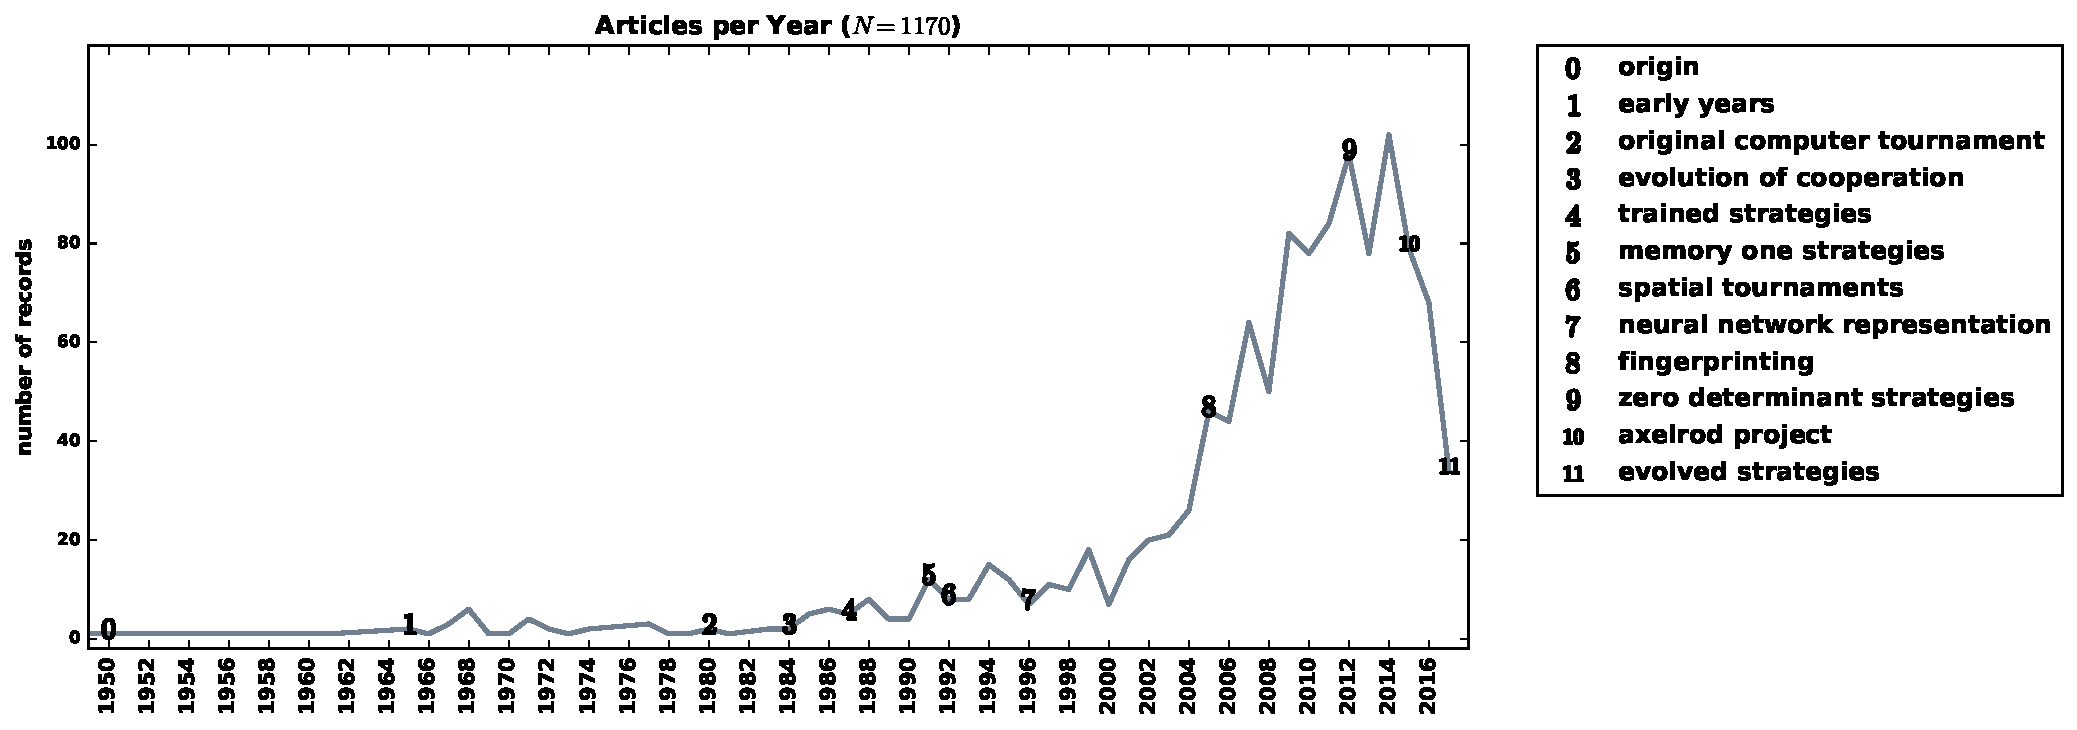
\includegraphics[width=.9\textwidth]{./assets/images/timeline.pdf}
    \caption{Line plot; \# of articles published on the PD 1950-2019.}\label{fig:timeseries}
\end{minipage}
\begin{minipage}{.45\textwidth}
    \centering
    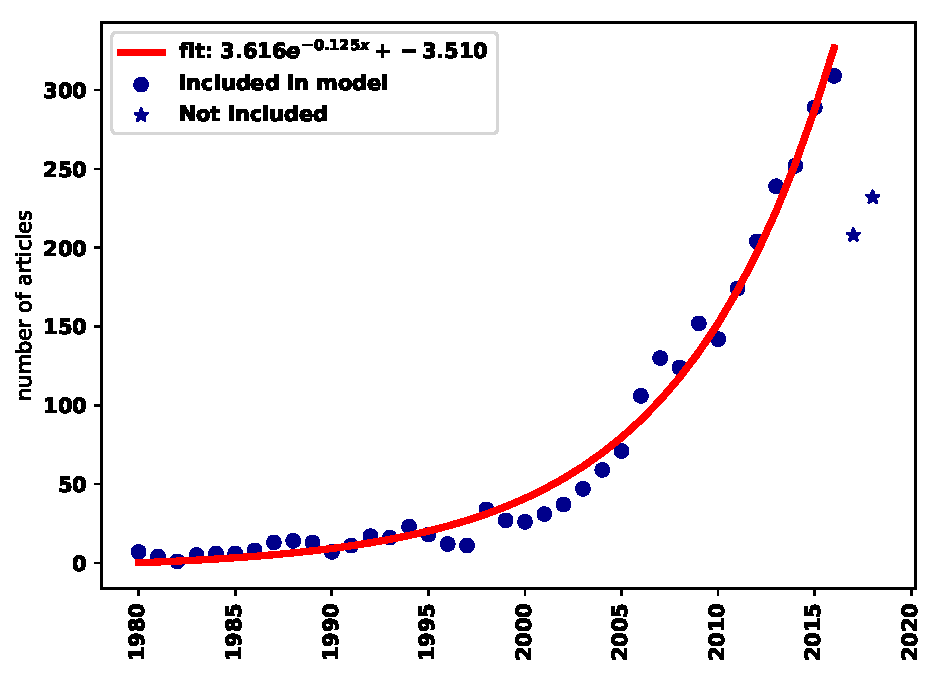
\includegraphics[width=.9\textwidth]{./assets/images/fitting.pdf}
    \caption{Scatter plot; \# of articles published on the PD 1980-2019.}\label{fig:fitting}
\end{minipage}
\end{figure}

\begin{figure}[!hbtp]
    \centering
    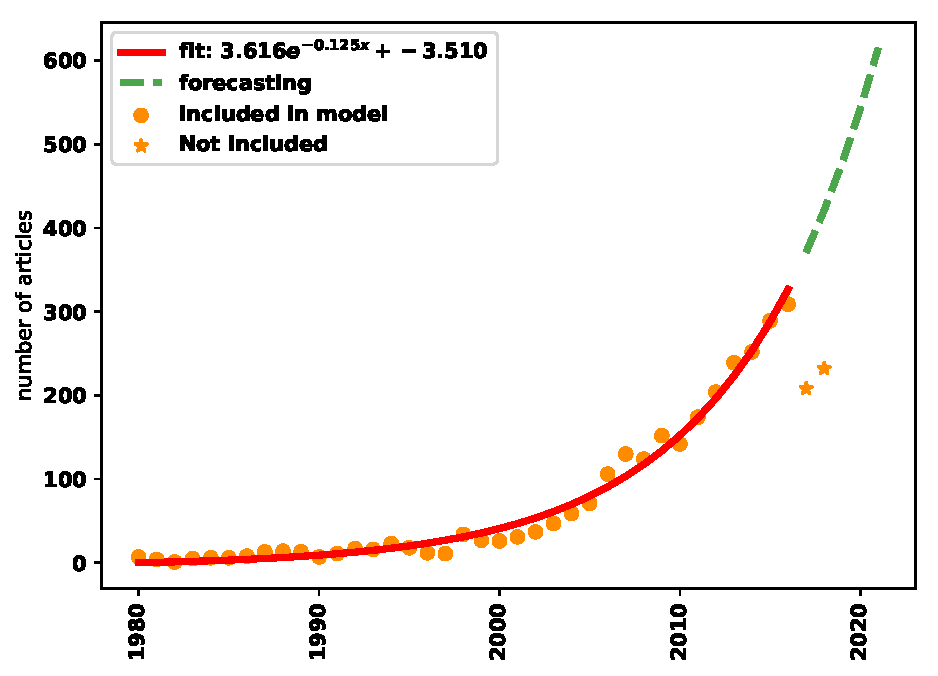
\includegraphics[width=.5\textwidth]{./assets/images/forecasting.pdf}
    \caption{Forecast for 2017-2022}\label{fig:forecasting}
\end{figure}

\begin{table}[!hbtp]
    \begin{center}
    \begin{tabular}{lr}
\toprule
{} &   Forecast \\
\midrule
1  &  27.301817 \\
2  &  24.500512 \\
3  &  26.490962 \\
4  &  26.208756 \\
5  &  27.004436 \\
6  &  27.288891 \\
7  &  27.815812 \\
8  &  28.227735 \\
9  &  28.694200 \\
10 &  29.134797 \\
\bottomrule
\end{tabular}

    \end{center}
    \caption{Forecasting the number of publications over the next 10 years.}
    \label{table:forecast}
\end{table}

Moreover, two sub fields of game theory have been chosen for this work; auction game and the
price of anarchy.

\begin{itemize}
    \item Auction theory; a branch of economics which deals with how
    people act in auction markets and researches the properties of auction markets.
    Game theory it's being used for years to study actions and the behaviour of
    the bidders~\cite{Shubik1971}. From the data tha have been collected here,
    the earliest entry is in 1974 (Figure~\ref{fig:timeseries_ag}).
    \item Price of Anarchy; is a concept in economics and game theory which
    measures how the efficiency of a system degrades due to selfish behaviour of
    its agents. There is a variety of such measures however the price of anarchy
    has attracted a lot of attention since its informal introduction in 2009
    by~\cite{Koutsoupias1999}. In Figure~\ref{fig:timeseries_pa} we see
    that the first entry in the data is around that time.
\end{itemize}

A summary of both data sets collected on both topics, in comparison to that of the
iterated prisoner's dilemma, is given by Table~\ref{table:summary_other_topics}.
The iterated prisoner's dilemma and auction theory are very well studied topics
that have been having publications for decades. A large number of articles have
been collected for both topics, 3091 and 34449 respectively. Though, auction
game have a larger number of articles, the iterated prisoner's dilemma appears
to have almost 300 more authors. Auction games have an overall average publication
of 90 articles compared to the IPD with 49.

Compared to these two topics the price of anarchy is a fairly recent topic.
Only a total of 747 articles have been collected, however it has a large number
of 1229 authors. Meaning that on average each paper had had at least two authors.
It has an overall average publication of 39 articles and no articles have been
collected from PLOS. Thus, no publications on the price of anarchy have been made
on the journal yet. The 50\% on auction games have been collected from arXiv,
and not articles have been added manually for the data sets for the two extra
sub fields.

\begin{table}[!hbtp]
        \centering
        \resizebox{\textwidth}{!}{
        \begin{tabular}{lrrllrrrrr}
\toprule
{} &  Num. Articles &  Num. Authors & Manual (\%) & PLOS (\%) &  Nature (\%) &  Springer (\%) &  IEEE (\%) &  arXiv (\%) &  Av. Yearly Publication \\
\midrule
Prisoner's Dilemma &           3089 &          5811 &       2.88 &     15.6 &       21.79 &         18.52 &      9.55 &      34.19 &                     NaN \\
Auction Games      &           3444 &          5362 &          - &        - &        5.89 &         37.63 &      7.46 &      51.36 &                     NaN \\
Price of Anarchy   &            746 &          1314 &          - &     1.74 &       24.66 &         38.07 &     30.70 &       8.85 &                     NaN \\
\bottomrule
\end{tabular}
}
        \caption{Measures of all three data sets.}\label{table:summary_other_topics}
\end{table}

\begin{figure}[!hbtp]
    \begin{minipage}{.45\textwidth}
        \centering
        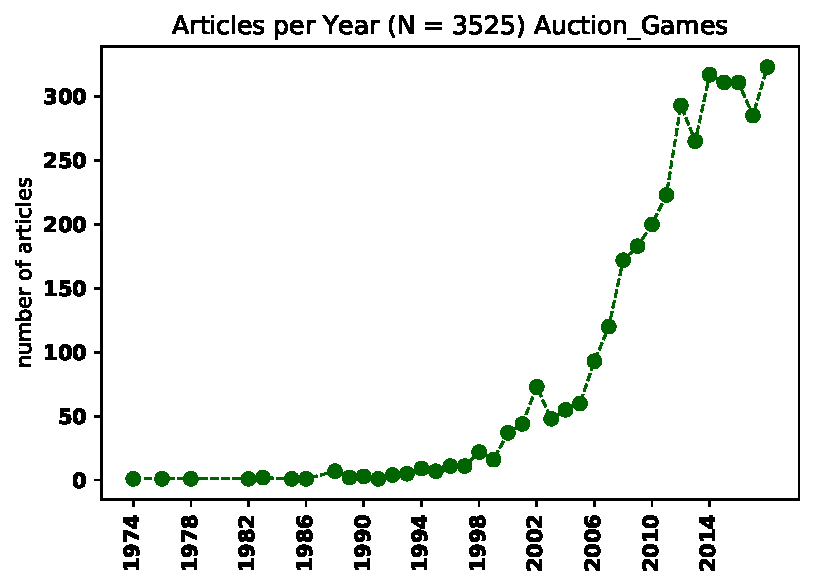
\includegraphics[width=\textwidth]{./assets/images/Auction_Games.pdf}
        \caption{Line plot showing the number of articles published on Auction Games.}\label{fig:timeseries_ag}
    \end{minipage}%
    \begin{minipage}{.45\textwidth}
        \centering
        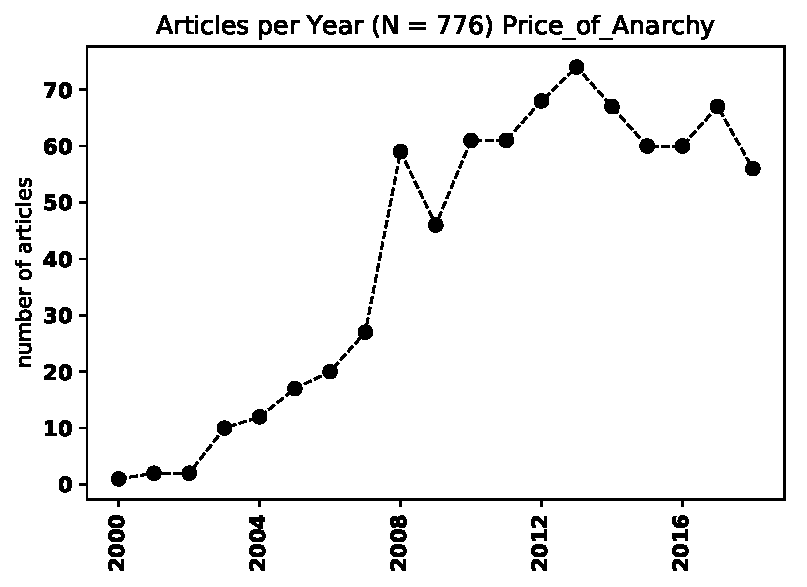
\includegraphics[width=\textwidth]{./assets/images/Price_of_Anarchy.pdf}
        \caption{Line plot showing the number of articles published on the Price of Anarchy.}\label{fig:timeseries_pa}
    \end{minipage}
    \end{figure}

In this section we have described the three data sets that we are going to use
in the following sections in order to identify collaborative behaviour and influence.
Two data sets of different topics are used for comparison reasons. The frequency of
articles and authors differs within the three data sets which is ideal.

\subsection{Methodology}\label{section:methodology}

As discussed in~\cite{youngblood2018}, bibliometrics or the statistical analysis
of published works (originally described by~\cite{pritchard1969}) 
have been used to support historical assumptions about the development of fields
\cite{raina1998}, identify connections between scientific growth and policy changes 
\cite{das2016}, and investigate the collaborative structure of an interdisciplinary
field~\cite{Liu2015}.
Most academic research is undertaken in the form of collaborative effort and as~\cite{Kyvik2017}
points out, it is rationale that two or more people have the potential to do better
as a group than individually. Collaboration in groups has a long tradition in experimental 
sciences and it has be proven to be productive according to~\cite{Etzkowitz1992}.
The number of collaborations can be very different between research fields and
understanding how collaborative a field is, it is not always an easy task.
Several studies tend to consider academic citations as a measure for these things.
A blog post published in Nature~\cite{nature_blog} argues that depending on citations
can often be misleading because the true number of citations can not be
known. Citations can be missed due to data entry errors, academics are influenced
by many more papers than they actually cite and several of the citations are
superficial.

A more recent approach to measure collaborative behaviour is to use the co
authorship network, as described in~\cite{Liu2015}. In this paper we build upon
the work done by~\cite{Liu2015} and also extend their methodology. Though in
\cite{Liu2015}, they considered a data set from a single source, Web of science,
our data have been collected from 5 different sources. Moreover, the collaborative
results of our analysis are compared to those of two different sub fields as well.
Co authorship networks have also been used in~\cite{youngblood2018} for classifying
topics of an interdisciplinary field. This was done using centrality measures,
which will be covered below, here we do not constrain our analysis to partitioning
the network but we use centrality measures in order to understand the influence
an author can have and can proceed by being part of the academic group.

So we can model relationship of authors within a field as a graph \(G\) with
a set \(V_G\) of nodes and \(E_G\) of edges. The set \(V_G\) represents the authors
and an edge connects two authors if and only if those authors have written together.
Co authorship networks have had several applications, including classifying topic
of an interdisciplinary field~\cite{youngblood2018}, but here we build upon the
work done by~\cite{Liu2015} on collaborative behaviour.
More specifically, here we explore the collaborativeness of the prisoner's dilemma
field, and we also extend the approach in order to understand influence;
how many connections are made possible because of an author. This possible
only because several graph theoretic measures can be used as proxies.
The co authorship network is constructed using the main data set described in
Section~\ref{section:preliminary_analysis} and the open source package Networkx
\cite{networkx}. The prisoner's dilemma network is denoted as \(G_1\) where the
number of unique authors \(|V(G_1)|\) is \authors and \(|E(G_1)|=\) \edges.
Note that the names of all authors were standardised to be their last name and
first initial (i.e. Martin A. Nowak to M.Nowak). This was done to avoid errors
such as Martin A. Nowak and Martin Nowak, being treated as a different person.
Networkx will also be used the following section to conduct our analysis.

Collaborativeness, will be analysed using measures such as, isolated nodes,
connected components, clustering coefficient, modularity and average degree.
These measures allow us to understand the number of connections author can have
and how strongly connected these people are. The number of isolated nodes allow
us to understand the how many nodes are not connected to another node, thus the
number of authors that had not had any known collaboration in the field.
The average degree denotes the average number of neighbours for each nodes, i.e.
the average number of collaborations between the authors and the number of largest
connected component represents the scale of the central cluster of the entire
network, as it will discussed in the analysis section. Clustering coefficient,
modularity and the degree distribution are also measured.
Clustering coefficient defined by,

\[C = \frac{3 \times \text{(number of triangle on the graph)}}{\text{number of connected triples of nodes}}\]

is a local measure of the degree to which nodes in a graph
tend to cluster together in a clique. It is precisely the probability that the collaborators
of an author also write together. In comparison, modularity is a global measure
designed to measure the strength of division of a network into modules. A high
value of modularity corresponds to a structure where authors meanly write
in groups and interact less with whole network. We will be using the Louvain method
described in~\cite{Blondel2008}.


Furthermore, the second part of the analysis focuses on the study of influence.
Networks are commonly dominated by one person who controls information flow and
people can still receive a great amount of information due to their position.
In this paper we aim to understand two things, (1) which people control the flow;
as in which people influence the field the most and (2) which are the authors that
gain the most from the influence of the field.
To measure these concepts we will be using graph theoretic metrics, more specifically
centrality measures. Centrality measures are often used to understand different
aspects fo social networks~\cite{Landherr2010}. In order to achieve that two
centrality measures that have been chosen were closeness and betweenness
centrality.

\begin{itemize}
    \item \textbf{Closeness} centrality of a node is the reciprocal of the average
    shortest path distance to the node, over all the rest reachable nodes.
    \item \textbf{Betweenness} centrality of a node is the sum of the fraction of
    all-pairs shortest paths that pass through the node.
\end{itemize}

In the next section we will be using all the metrics discussed here to
provide insights on the field, this will done also by comparing to the PD network
to two other fields of game theory as well as exploring the progress of the
network over time.

\subsection{Analysis of co authorship network}\label{section:results}

As mentioned previously, \(G_1\) denotes the co authorship network of iterated
prisoner's dilemma. The open source software Gephi~\cite{ICWSM09154} has been used
to plot the networks of this work, more specifically \(G_1\) is given by Figure.
It is evident that our network is disjoint, which is only natural as many authors
write academic articles on their own. More specifically, a total of \isolated authors,
have had single author publications, which corresponds to the \isolatedpercentage (\%)
of authors in \(G_1\). There are a total of \connectedcomponents and the largest
one has a size of \largestcc. The largest connected component is shown in
Figure.
The network as a clustering coefficient of \clustering, thus you are 68\% likely
to write with a collaborators co author. Overall the networks have an average
degree of \avdegree, meaning that the average publication on the field has
4 authors. The distribution of the degrees, Figure~\ref{fig:degree_distr_pd},
indicates that thought the average is 4 there are authors with far more connections,
the largest one being around 30.

\begin{figure}[!hbtp]
    \centering
    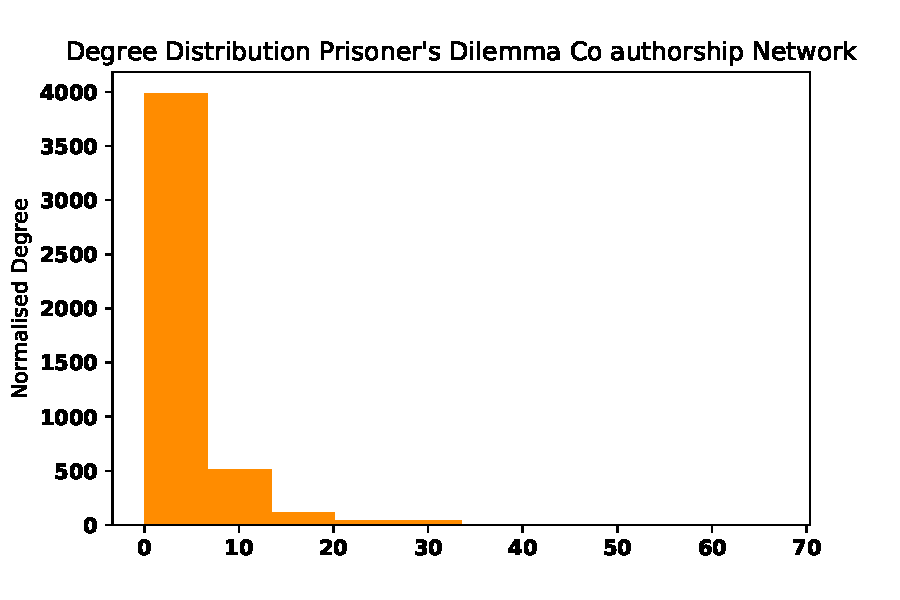
\includegraphics[width=.5\textwidth]{./assets/images/pd_degree_distribution.pdf}
    \caption{Degree distribution for network \(G_1\).}\label{fig:degree_distr_pd}
\end{figure}

\begin{figure}[!hbtp]
    \centering
    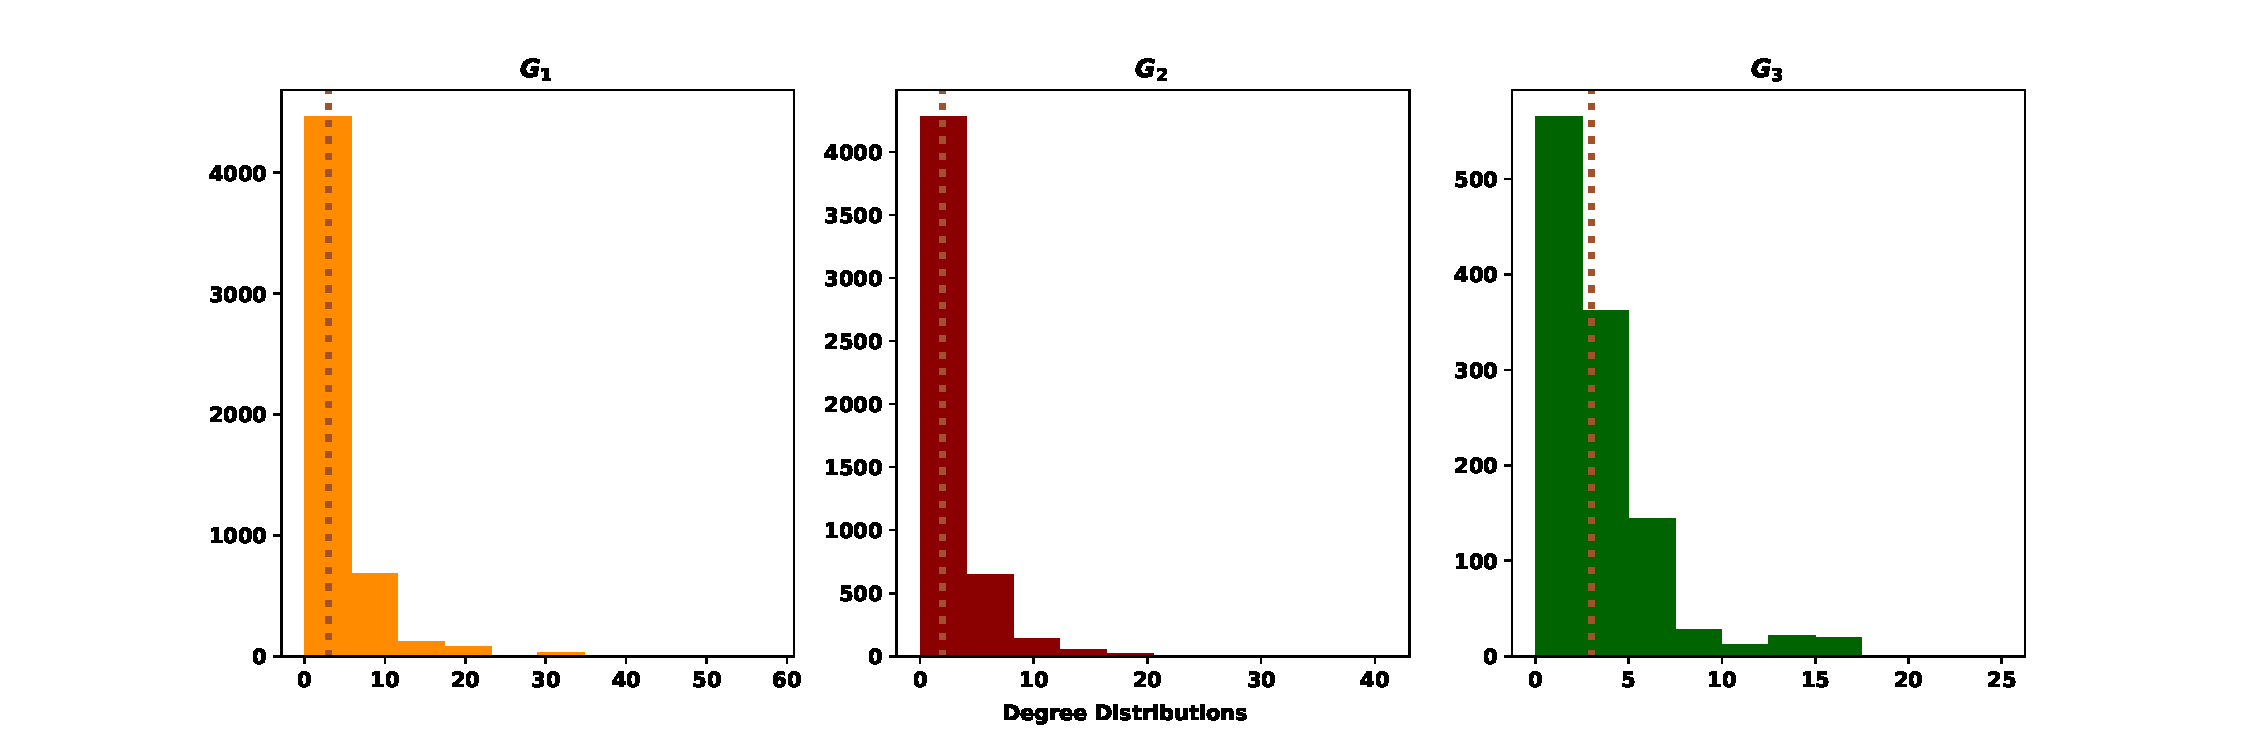
\includegraphics[width=\textwidth]{./assets/images/networks_ditributions.pdf}
    \caption{Degree distribution for networks \(G_1\)\-\(G_3\).}\label{fig:degree_distrs}
\end{figure}

How does these compare to other fields and more specifically to other fields of
game theory? A summary of the two graphs, which be denoted as \(G_2\) for auction
games and \(G_3\) for the price of anarchy, are given by Figure.
A summary of metrics and for all three co authorship networks is given by
Table~\ref{table:summary_other_networks}. The following remarks can be made
from Table~\ref{table:summary_other_networks}.

\begin{itemize}
    \item Comparing to another well studied topic (\(G_2\)), the co authorship
    network \(G_1\) appears to be more modular. This is due the high values of
    modularity, connected components and clustering coefficient. Authors in \(G_1\)
    tend to write in teams, separated from the main cluster and it's very likely
    to create smaller clusters of 3. Compared that \(G_2\) has a smaller number
    of connected component but the the main cluster has a bigger size.
    \item In the more recent topic price of anarchy (\(G_3\)) there are hardly
    any people that have published a paper alone. There is already a small community
    that is connected with a main cluster of 421 authors. The network is also very
    modular. Indicating that people that are not connected to the main cluster
    are in smaller connected components. There is even higher clustering coefficient
    compared to the rest of networks so these connected components are very likely
    of size 3, which is also indicated by the degree distribution of \(G_3\)
    (Figure~\ref{fig:degree_distrs}).
    \item Shown in Figure~\ref{fig:degree_distrs} the degree distributions of
    \(G_1\) and \(G_2\) are more skewed to the left, though there are some cases
    of high degree (\(> 20\)) this could be due the size of the networks and
    respectively the size of the main clusters.
\end{itemize}

\begin{table}[!hbtp]
    \centering
    \resizebox{\textwidth}{!}{
    \begin{tabular}{lrrrrrrrrrr}
\toprule
{} &  \# Nodes &  \# Edges &  \# Isolated nodes &  \% Isolated nodes &  \# Connected components &  Size of largest component &  Av. degree &  \# Communities &  Modularity &  Clustering coeff \\
\midrule
$G$              &     4221 &     7642 &               338 &               8.0 &                    1157 &                        796 &       3.621 &           1177 &    0.965264 &             0.666 \\
$\bar{G}$        &      796 &     2214 &                 0 &               0.0 &                       1 &                        796 &       5.563 &             29 &    0.840138 &             0.773 \\
Auction Games    &     5362 &     7861 &               453 &               8.4 &                    1469 &                       1348 &       2.932 &           1493 &    0.957238 &             0.599 \\
Price of Anarchy &     1315 &     1952 &               165 &              12.5 &                     406 &                        221 &       2.969 &            414 &    0.964498 &             0.626 \\
\bottomrule
\end{tabular}
}
    \caption{Network metrics for \(G_1, G_2, G_3\).}\label{table:summary_other_networks}
\end{table}

The growth of collaborativeness behaviour can also be studied. The cumulative graphs
for has been computed. There are a total of 64 graphs, for 64 periods starting
from 1954. All the collaborative metrics have been calculated for each period
and they are given in Table~\ref{table:coll_cumulative}.
In Figure~\ref{fig:nodes_cumu_pd}, the number of nodes over time have been plotted. More specifically,
we plot the normalised number of nodes which is calculated by dividing with
the total number of nodes, in \(G_1\) case that is \authors. A steep increase,
appears to be happening after 2000, though this could indicate a specific
thing that happened only in \(G_1\), Figure~\ref{fig:nodes_cumu} argues with that.
Compared to both \(G_2\) and \(G_3\) there is an increase in the number of authors
since 2000.

\begin{figure}[!hbtp]
    \begin{minipage}{.45\textwidth}
        \centering
        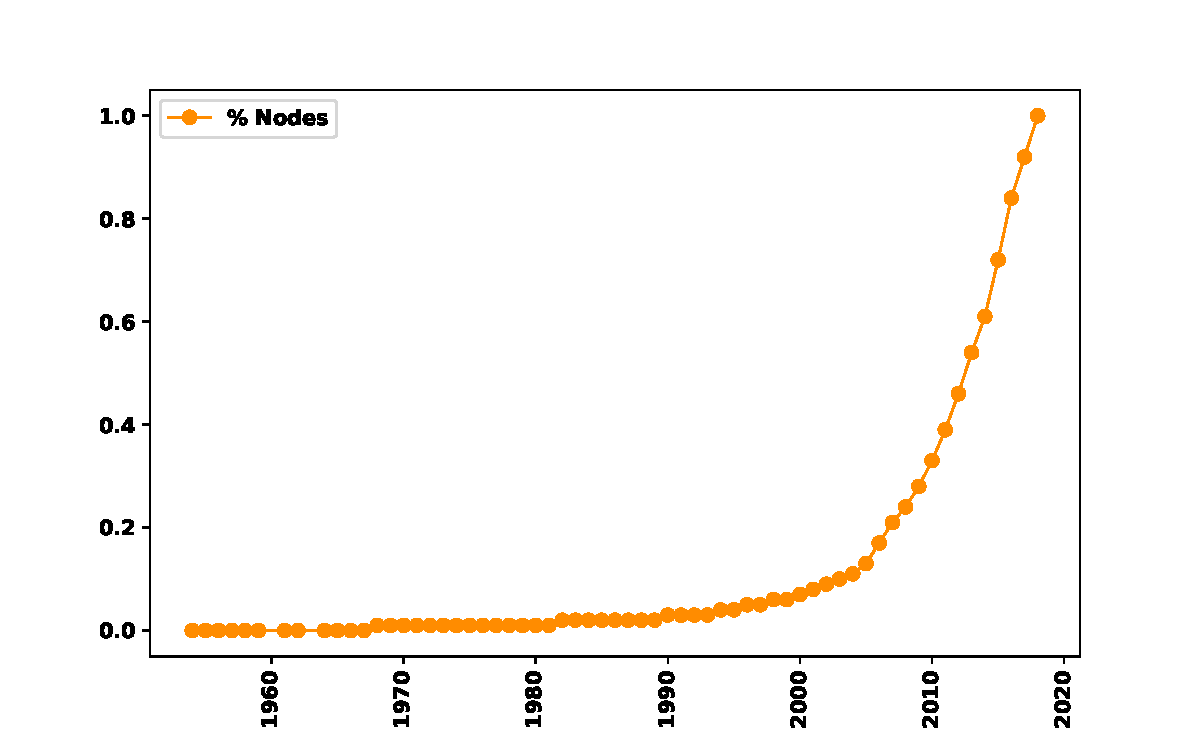
\includegraphics[width=\textwidth]{./assets/images/nodes_percentage_over_time.pdf}
        \caption{Normalized \# Nodes over time for \(G_1\).}\label{fig:nodes_cumu_pd}
    \end{minipage}%
    \begin{minipage}{.45\textwidth}
        \centering
        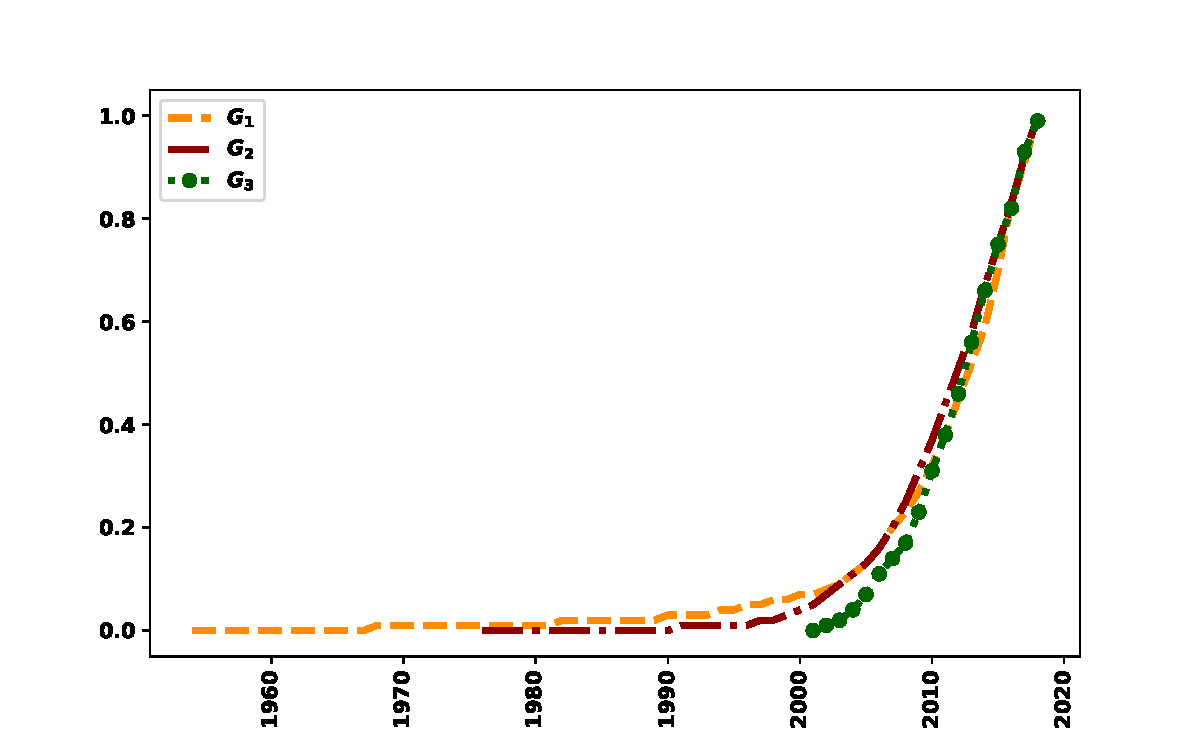
\includegraphics[width=\textwidth]{./assets/images/percentage_networks_nodes.pdf}
        \caption{Normalized \# Nodes over time for all networks.}\label{fig:nodes_cumu}
    \end{minipage}
\end{figure}

The average degree over time for all three networks is given Figure~\ref{fig:degree_distr_cumu}.
Thought auction game theory and the prisoners' dilemma have been for different
time periods we can see that the follow a similar trend. A small peek after the
first years of publications followed by a steady increase ever since with a highest
value of an average degree of 4. Price of anarchy as a similar trend but suffered of
a small decrease around 2003.

\begin{figure}[!hbtp]
    \centering
    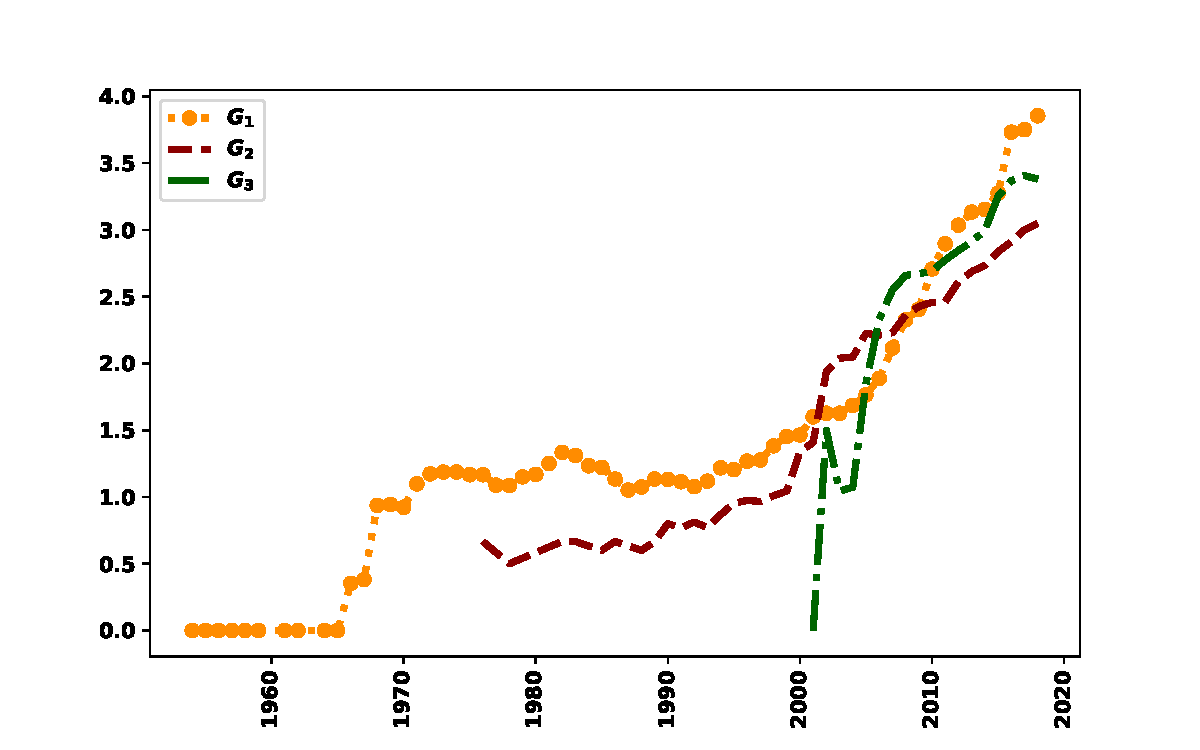
\includegraphics[width=.7\textwidth]{./assets/images/degrees_over_time.pdf}
    \caption{Degree distribution for network \(G_1\).}\label{fig:degree_distr_cumu}
\end{figure}
    
% Moreover, Table provides a clearer insight on the field chaning over time.
% With a time 5 years we un contructed the cumulatice co authror ship network
% and Table summarizes all the metrics as discussed all ready.

\begin{table}[!hbtp]
    \centering
    \begin{adjustbox}{totalheight=\textheight-2\baselineskip}
    \begin{tabular}{lrrrrrrrllr}
\toprule
{} &  \# Nodes &  \# Edges &  \# Isolated nodes &  \% Isolated nodes &  \# Connected components &  Size of largest component &  Av. degree & \# Communities & Modularity &  Clustering coeff \\
\midrule
1954 - 1950 &        3 &        0 &                 3 &             100.0 &                       3 &                          1 &       0.000 &             - &          - &             0.000 \\
1954 - 1955 &        2 &        0 &                 2 &             100.0 &                       2 &                          1 &       0.000 &             - &          - &             0.000 \\
1955 - 1956 &        3 &        0 &                 3 &             100.0 &                       3 &                          1 &       0.000 &             - &          - &             0.000 \\
1956 - 1957 &        4 &        0 &                 4 &             100.0 &                       4 &                          1 &       0.000 &             - &          - &             0.000 \\
1957 - 1958 &        6 &        0 &                 6 &             100.0 &                       6 &                          1 &       0.000 &             - &          - &             0.000 \\
1958 - 1959 &        7 &        0 &                 7 &             100.0 &                       7 &                          1 &       0.000 &             - &          - &             0.000 \\
1959 - 1961 &        7 &        0 &                 7 &             100.0 &                       7 &                          1 &       0.000 &             - &          - &             0.000 \\
1961 - 1962 &        8 &        0 &                 8 &             100.0 &                       8 &                          1 &       0.000 &             - &          - &             0.000 \\
1962 - 1964 &        9 &        0 &                 9 &             100.0 &                       9 &                          1 &       0.000 &             - &          - &             0.000 \\
1964 - 1965 &       10 &        0 &                10 &             100.0 &                      10 &                          1 &       0.000 &             - &          - &             0.000 \\
1965 - 1966 &       17 &        3 &                11 &              64.7 &                      14 &                          2 &       0.353 &            14 &   0.666667 &             0.000 \\
1966 - 1967 &       21 &        4 &                13 &              61.9 &                      17 &                          2 &       0.381 &            17 &       0.75 &             0.000 \\
1967 - 1968 &       32 &       15 &                13 &              40.6 &                      21 &                          5 &       0.938 &            21 &   0.684444 &             0.135 \\
1968 - 1969 &       36 &       17 &                16 &              44.4 &                      24 &                          6 &       0.944 &            24 &   0.629758 &             0.139 \\
1969 - 1970 &       39 &       18 &                17 &              43.6 &                      26 &                          6 &       0.923 &            26 &   0.666667 &             0.128 \\
1970 - 1971 &       51 &       28 &                18 &              35.3 &                      31 &                          6 &       1.098 &            31 &   0.826531 &             0.275 \\
1971 - 1972 &       58 &       34 &                19 &              32.8 &                      34 &                          6 &       1.172 &            34 &   0.866782 &             0.345 \\
1972 - 1973 &       59 &       35 &                18 &              30.5 &                      34 &                          6 &       1.186 &            34 &   0.873469 &             0.339 \\
1973 - 1974 &       59 &       35 &                18 &              30.5 &                      34 &                          6 &       1.186 &            34 &   0.873469 &             0.339 \\
1974 - 1975 &       60 &       35 &                19 &              31.7 &                      35 &                          6 &       1.167 &            35 &   0.873469 &             0.333 \\
1975 - 1976 &       60 &       35 &                19 &              31.7 &                      35 &                          6 &       1.167 &            35 &   0.873469 &             0.333 \\
1976 - 1977 &       68 &       37 &                23 &              33.8 &                      41 &                          6 &       1.088 &            41 &   0.885318 &             0.294 \\
1977 - 1978 &       70 &       38 &                23 &              32.9 &                      42 &                          6 &       1.086 &            42 &   0.890582 &             0.286 \\
1978 - 1979 &       73 &       42 &                23 &              31.5 &                      42 &                          6 &       1.151 &            42 &   0.893424 &             0.292 \\
1979 - 1980 &       77 &       45 &                25 &              32.5 &                      44 &                          6 &       1.169 &            44 &   0.899753 &             0.307 \\
1980 - 1981 &       80 &       50 &                26 &              32.5 &                      45 &                          6 &       1.250 &            45 &     0.8928 &             0.318 \\
1981 - 1982 &       84 &       56 &                26 &              31.0 &                      46 &                          6 &       1.333 &            46 &   0.903061 &             0.350 \\
1982 - 1983 &       87 &       57 &                27 &              31.0 &                      48 &                          6 &       1.310 &            48 &   0.906125 &             0.338 \\
1983 - 1984 &       94 &       58 &                32 &              34.0 &                      54 &                          6 &       1.234 &            54 &   0.909037 &             0.313 \\
1984 - 1985 &       95 &       58 &                33 &              34.7 &                      55 &                          6 &       1.221 &            55 &   0.909037 &             0.309 \\
1985 - 1986 &      104 &       59 &                40 &              38.5 &                      63 &                          6 &       1.135 &            63 &   0.911807 &             0.283 \\
1986 - 1987 &      116 &       61 &                48 &              41.4 &                      73 &                          6 &       1.052 &            73 &   0.916958 &             0.253 \\
1987 - 1988 &      121 &       65 &                48 &              39.7 &                      75 &                          6 &       1.074 &            75 &   0.924497 &             0.268 \\
1988 - 1989 &      134 &       76 &                47 &              35.1 &                      80 &                          6 &       1.134 &            80 &   0.937673 &             0.272 \\
1989 - 1990 &      145 &       82 &                49 &              33.8 &                      86 &                          6 &       1.131 &            86 &   0.944676 &             0.272 \\
1990 - 1991 &      158 &       88 &                53 &              33.5 &                      94 &                          6 &       1.114 &            94 &   0.950413 &             0.268 \\
1991 - 1992 &      169 &       91 &                59 &              34.9 &                     102 &                          6 &       1.077 &           102 &   0.953025 &             0.251 \\
1992 - 1993 &      186 &      104 &                62 &              33.3 &                     110 &                          6 &       1.118 &           110 &    0.95932 &             0.266 \\
1993 - 1994 &      220 &      134 &                72 &              32.7 &                     127 &                          6 &       1.218 &           127 &   0.965471 &             0.317 \\
1994 - 1995 &      239 &      144 &                74 &              31.0 &                     137 &                          6 &       1.205 &           137 &   0.969329 &             0.304 \\
1995 - 1996 &      257 &      163 &                77 &              30.0 &                     145 &                          6 &       1.268 &           145 &   0.970831 &             0.318 \\
1996 - 1997 &      279 &      178 &                81 &              29.0 &                     156 &                          6 &       1.276 &           156 &   0.974309 &             0.336 \\
1997 - 1998 &      311 &      215 &                65 &              20.9 &                     160 &                          6 &       1.383 &           160 &   0.979773 &             0.354 \\
1998 - 1999 &      329 &      239 &                58 &              17.6 &                     162 &                          6 &       1.453 &           162 &   0.981741 &             0.376 \\
1999 - 2000 &      373 &      273 &                67 &              18.0 &                     183 &                          6 &       1.464 &           183 &   0.983778 &             0.387 \\
2000 - 2001 &      400 &      320 &                54 &              13.5 &                     184 &                          7 &       1.600 &           184 &   0.983066 &             0.410 \\
2001 - 2002 &      450 &      366 &                61 &              13.6 &                     206 &                          7 &       1.627 &           206 &   0.984547 &             0.418 \\
2002 - 2003 &      509 &      414 &                58 &              11.4 &                     229 &                          7 &       1.627 &           229 &   0.987083 &             0.421 \\
2003 - 2004 &      580 &      489 &                58 &              10.0 &                     253 &                         10 &       1.686 &           253 &   0.988052 &             0.429 \\
2004 - 2005 &      679 &      599 &                57 &               8.4 &                     284 &                         19 &       1.764 &           284 &    0.98891 &             0.463 \\
2005 - 2006 &      854 &      806 &                66 &               7.7 &                     342 &                         21 &       1.888 &           342 &   0.990724 &             0.496 \\
2006 - 2007 &     1056 &     1117 &                76 &               7.2 &                     402 &                         24 &       2.116 &           402 &   0.989663 &             0.527 \\
2007 - 2008 &     1255 &     1460 &                85 &               6.8 &                     454 &                         32 &       2.327 &           455 &   0.989753 &             0.549 \\
2008 - 2009 &     1462 &     1759 &               104 &               7.1 &                     520 &                         56 &       2.406 &           521 &   0.987517 &             0.550 \\
2009 - 2010 &     1700 &     2301 &               114 &               6.7 &                     581 &                         99 &       2.707 &           584 &   0.979084 &             0.571 \\
2010 - 2011 &     2040 &     2954 &               121 &               5.9 &                     665 &                        121 &       2.896 &           668 &   0.980477 &             0.603 \\
2011 - 2012 &     2422 &     3676 &               126 &               5.2 &                     756 &                        210 &       3.036 &           759 &   0.979196 &             0.629 \\
2012 - 2013 &     2807 &     4398 &               138 &               4.9 &                     843 &                        330 &       3.134 &           849 &   0.976132 &             0.639 \\
2013 - 2014 &     3199 &     5044 &               148 &               4.6 &                     942 &                        406 &       3.153 &           950 &   0.974968 &             0.651 \\
2014 - 2015 &     3798 &     6221 &               159 &               4.2 &                    1064 &                        514 &       3.276 &          1074 &   0.976242 &             0.668 \\
2015 - 2016 &     4472 &     8344 &               169 &               3.8 &                    1184 &                        614 &       3.732 &          1198 &   0.975233 &             0.690 \\
2016 - 2017 &     4925 &     9235 &               173 &               3.5 &                    1274 &                        703 &       3.750 &          1292 &   0.976353 &             0.700 \\
2017 - 2018 &     5385 &    10379 &               176 &               3.3 &                    1356 &                        815 &       3.855 &          1369 &   0.977318 &             0.708 \\
\bottomrule
\end{tabular}
}
    \caption{Collaborativeness metrics for cumulative graphs.}\label{table:coll_cumulative}
\end{adjustbox}
\end{table}

The influence of the networks were explored using centrality measures. For \(G_1\)
the most central author based on closeness and betweenness are given by Tables
respectively.


\begin{figure}[!hbtp]
    \begin{minipage}{.45\textwidth}
        \centering
        \centering
        \begin{tabular}{llr}
\toprule
{} &       Name &  Betweeness \\
\midrule
1  &    M. Perc &    0.018903 \\
2  &    Z. Wang &    0.015962 \\
3  &    L. Wang &    0.014842 \\
4  &   Y. Zhang &    0.013178 \\
5  &   M. Nowak &    0.011588 \\
6  &    H. Wang &    0.008221 \\
7  &    Y. Chen &    0.008070 \\
8  &      Y. Li &    0.007993 \\
9  &  Y. Moreno &    0.007132 \\
10 &  N. Masuda &    0.006087 \\
\bottomrule
\end{tabular}

        \caption{Ten most influenced authors in \(G_1\).}\label{table:central_authors}
    \end{minipage}%
    \begin{minipage}{.45\textwidth}
        \centering
        \begin{tabular}{llr}
\toprule
{} &             Name &  Closeness \\
\midrule
1  &      Matjaz Perc &   0.061854 \\
2  &     Yamir Moreno &   0.057163 \\
3  &        Long Wang &   0.056003 \\
4  &        Zhen Wang &   0.055938 \\
5  &  Attila Szolnoki &   0.055367 \\
6  &    Luo-Luo Jiang &   0.053405 \\
7  &    Arne Traulsen &   0.053153 \\
8  &     Cheng-Yi Xia &   0.052018 \\
9  &  Valerio Capraro &   0.051651 \\
10 &    Angel Sanchez &   0.051523 \\
\bottomrule
\end{tabular}

        \caption{Authors that gain the most influence in \(G_1\).}\label{table:central_authors_cc}
    \end{minipage}
\end{figure}

\begin{figure}[!hbtp]
    \centering
    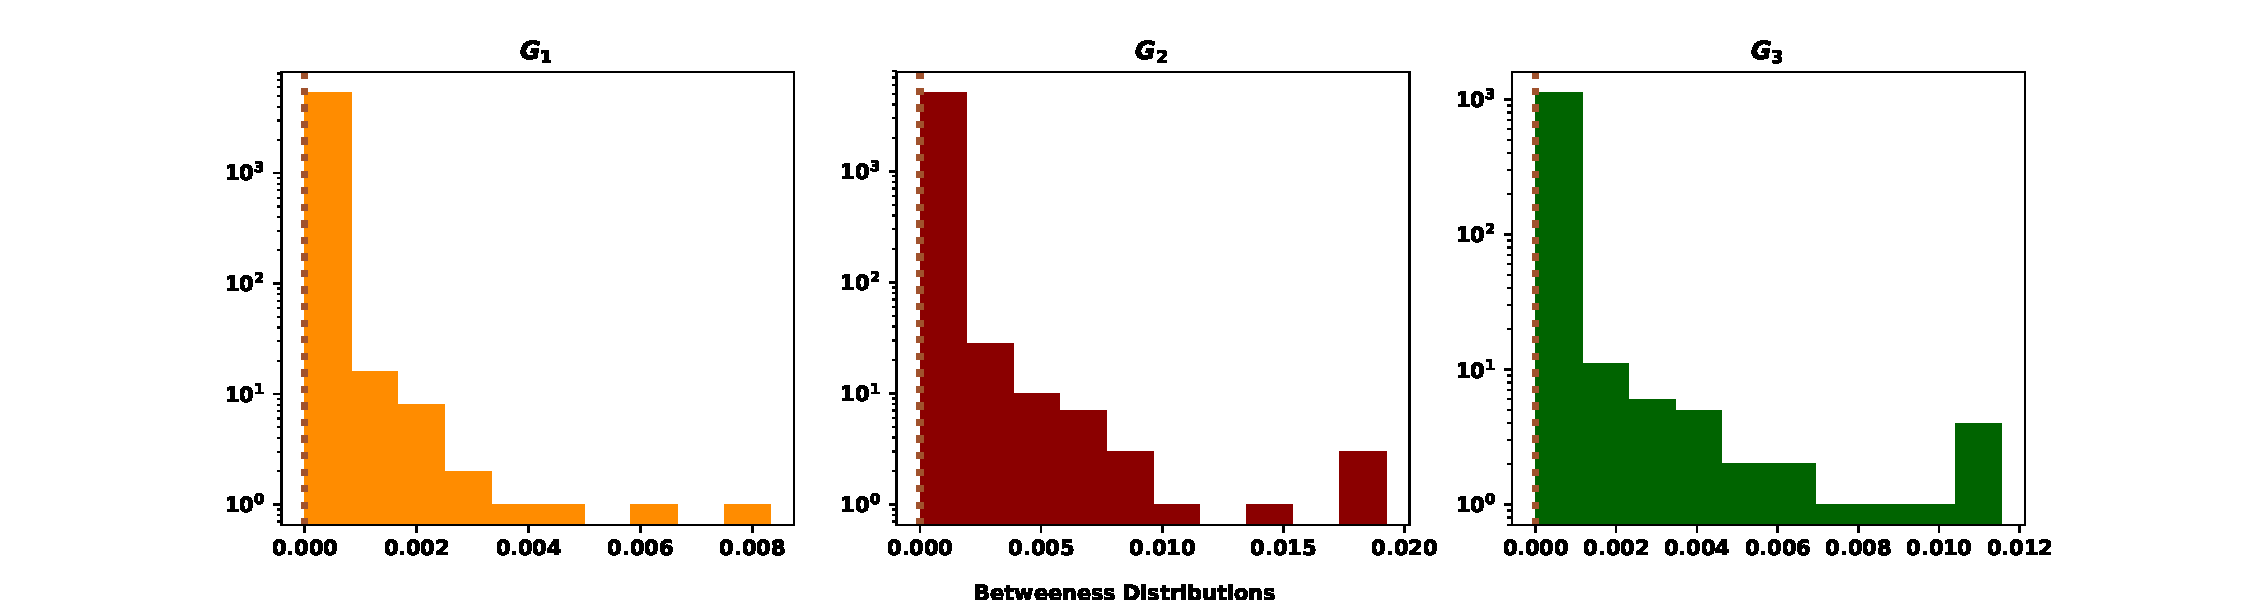
\includegraphics[width=\textwidth]{./assets/images/betweeness_distributions.pdf}
    %\caption{Degree distribution for network \(G_1\).}\label{fig:degree_distr_cumu}
\end{figure}

\begin{figure}[!hbtp]
    \centering
    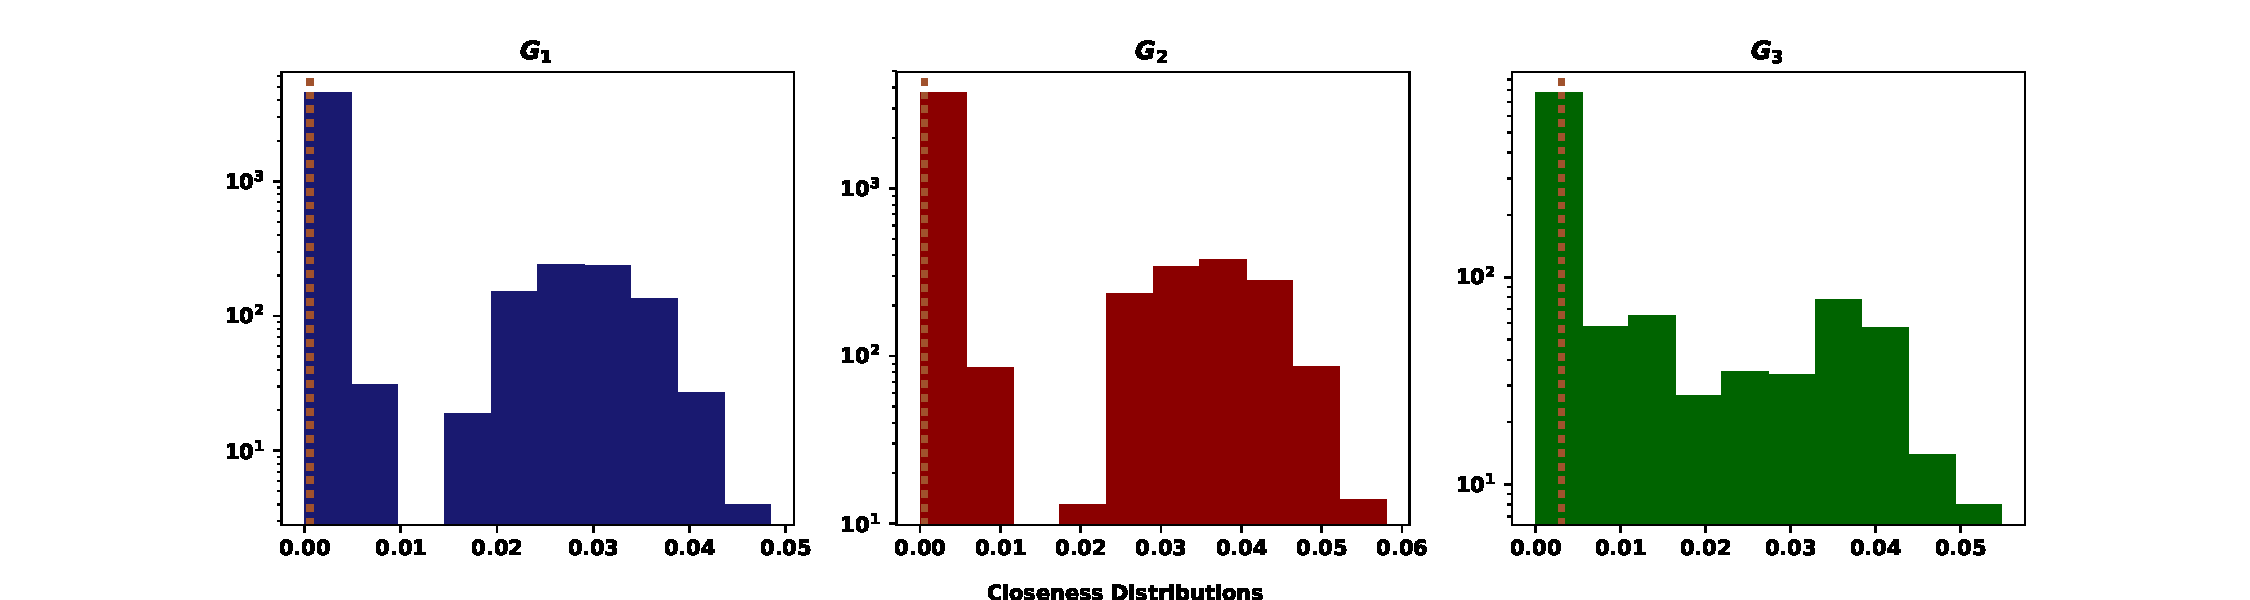
\includegraphics[width=\textwidth]{./assets/images/closeness_distributions.pdf}
    %\caption{Degree distribution for network \(G_1\).}\label{fig:closeness_distributions.pdf}
\end{figure}

\begin{figure}[!hbtp]
    \centering
    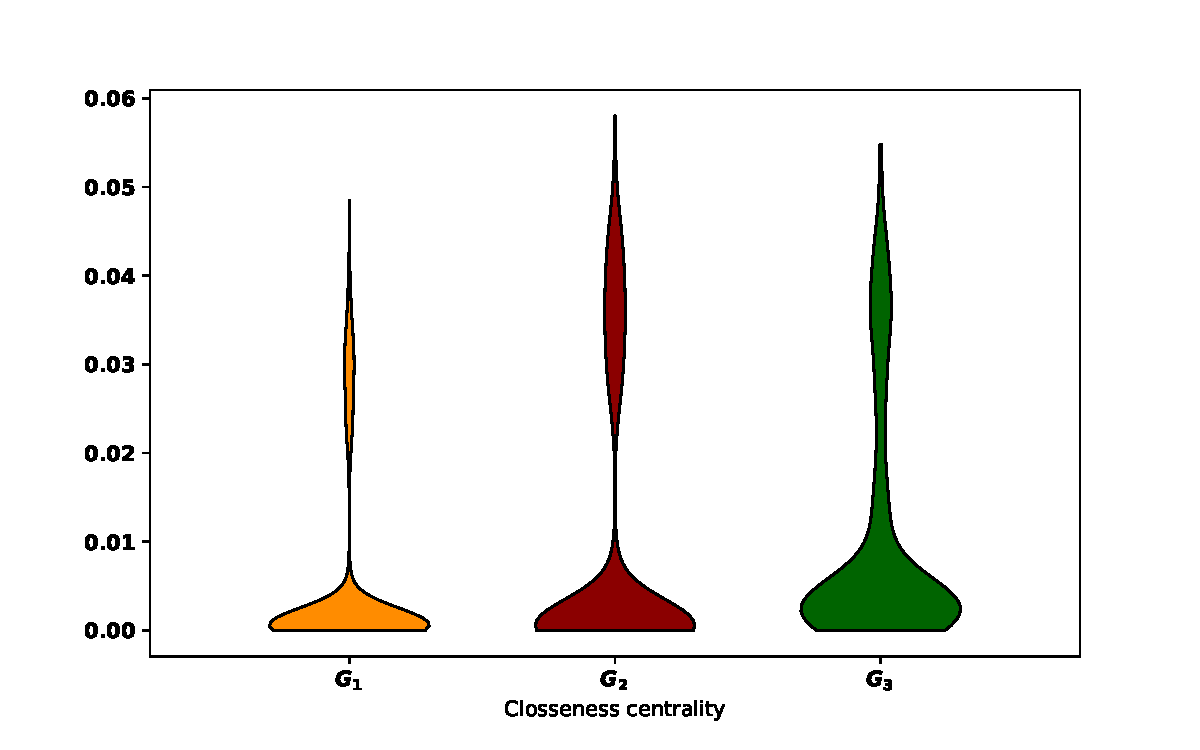
\includegraphics[width=\textwidth]{./assets/images/closeness_violins.pdf}
    %\caption{Degree distribution for network \(G_1\).}\label{fig:closeness_distributions.pdf}
\end{figure}


\subsection{Conclusion}

\newpage
\bibliographystyle{plain}
\bibliography{bibliography.bib}
\end{document}
